\documentclass[12pt]{article}
% Load packages
\usepackage{url}  % Formatting web addresses
\usepackage{ifthen}  % Conditional
\usepackage{multicol}   %Columns
\usepackage[utf8]{inputenc} %unicode support
\usepackage{amsmath}
\usepackage{amssymb}
\usepackage{epsfig}
\usepackage{epstopdf}
\usepackage{graphicx}
\usepackage[margin=0.1pt,font=footnotesize,labelfont=bf]{caption}
\usepackage{setspace}
%\usepackage{longtable}
\usepackage{colortbl}
%\usepackage{palatino,lettrine}
%\usepackage{times}
%\usepackage[applemac]{inputenc} %applemac support if unicode package fails
%\usepackage[latin1]{inputenc} %UNIX support if unicode package fails
\usepackage[wide]{sidecap}
%\usepackage[authoryear,round,comma,sort&compress]{natbib}
\usepackage[square,sort,comma,numbers,sort&compress]{natbib}
%\usepackage[authoryear,round]{natbib}
\usepackage{supertabular}
\usepackage{simplemargins}
\usepackage{fullpage}
\usepackage{comment}
\usepackage{lineno}
%\usepackage{chicago}
\usepackage{textcomp}
\usepackage{multirow}
\usepackage{amsmath}
\DeclareMathOperator*{\argmin}{\arg\!\min}

\usepackage{algorithm2e}
%\usepackage[space]{cite}
\urlstyle{rm}

%\textwidth = 6.50 in
%\textheight = 9.5 in
%\oddsidemargin =  0.0 in
%\evensidemargin = 0.0 in
%\topmargin = -0.50 in
%\headheight = 0.0 in
%\headsep = 0.25 in
%\parskip = 0.15in
%\linespread{1.75}
\doublespace

%\bibliographystyle{chicago}
\bibliographystyle{plos2009}

\makeatletter
\renewcommand\subsection{\@startsection
	{subsection}{2}{0mm}
	{-0.05in}
	{-0.5\baselineskip}
	{\normalfont\normalsize\bfseries}}
\renewcommand\subsubsection{\@startsection
	{subsubsection}{2}{0mm}
	{-0.05in}
	{-0.5\baselineskip}
	{\normalfont\normalsize\itshape}}
\renewcommand\section{\@startsection
	{subsection}{2}{0mm}
	{-0.2in}
	{0.05\baselineskip}
	{\normalfont\large\bfseries}}
\renewcommand\paragraph{\@startsection
	{paragraph}{2}{0mm}
	{-0.05in}
	{-0.5\baselineskip}
	{\normalfont\normalsize\itshape}}
\makeatother

%Review style settings
%\newenvironment{bmcformat}{\begin{raggedright}\baselineskip20pt\sloppy\setboolean{publ}{false}}{\end{raggedright}\baselineskip20pt\sloppy}

%Publication style settings

% Single space'd bib -
\setlength\bibsep{0pt}

\renewcommand{\rmdefault}{phv}\renewcommand{\sfdefault}{phv}
\newcommand{\norm}[1]{\left\lVert#1\right\rVert}

% Change the number format in the ref list -
\renewcommand{\bibnumfmt}[1]{#1.}

% Change Figure to Fig.
\renewcommand{\figurename}{Fig.}

% Begin ...
\begin{document}
\begin{titlepage}
{\par\centering\textbf{\Large {Dynamic Optimization with Particle Swarms (DOPS): A meta-heuristic for parameter estimation in biochemical models}}}
\vspace{0.05in}
{\par \centering \large{Adithya Sagar, Christine Shoemaker$^{\dag}$ and Jeffrey D. Varner$^{*}$}}
\vspace{0.10in}
{\par \centering {School of Chemical and Biomolecular Engineering}}
{\par \centering {$^{\dag}$School of Civil and Environmental Engineering}}
{\par \centering {Cornell University, Ithaca NY 14853}}
\vspace{0.1in}
{\par \centering \textbf{Running Title:}~Parameter estimation in biochemical models}
\vspace{0.1in}
{\par \centering \textbf{To be submitted:}~\emph{PLoS ONE}}
\vspace{0.5in}
{\par \centering $^{*}$Corresponding author:}
{\par \centering Jeffrey D. Varner,}
{\par \centering Associate Professor, School of Chemical and Biomolecular Engineering,}
{\par \centering 244 Olin Hall, Cornell University, Ithaca NY, 14853}
{\par \centering Email: jdv27@cornell.edu}
{\par \centering Phone: (607) 255 - 4258}
{\par \centering Fax: (607) 255 - 9166}
\end{titlepage}
\date{}
\thispagestyle{empty}
\pagebreak
%%%%%%%%%%%%%%%%%%%%%%%%%%%%%%%%%%%%%%%%%%%%%%%%%%%%%%%%%%%%%%%%%%%%%%%%%%%%%%%%%%%%%%%%%%%%%%%%%%%%%%%%%%%
%%%%%%%%%%%%%%%%%%%%%%%%%%%%%%%%%%%%%%%%%%%%%%%%%%%%%%%%%%%%%%%%%%%%%%%%%%%%%%%%%%%%%%%%%%%%%%%%%%%%%%%%%%%
\section*{Abstract}
Mathematical modeling is a powerful tool to analyze, and ultimately design biochemical networks.
However, the estimation of biochemical model parameters is a significant challenge.
Parameter estimation in biochemical models typically involves expensive function evaluations and noisy data, making it difficult to quickly obtain optimal solutions.
Biochemical models often also have many local extrema which further complicates parameter estimation.
Toward these challenges, we developed Dynamic Optimization with Particle Swarms (DOPS), a novel global meta-heuristic that combined features of multi-swarm particle swarm optimization with dynamically dimensioned search (DDS).
DOPS uses a multi-swarm particle swarm optimization technique to generate candidate solution vectors, the best of which is greedily updated using dynamically dimensioned search.
We tested the performance of DOPS on a model of human coagulation cascade.
We performed $\mathcal{T}$ = 25 trials with $\mathcal{N}$ = 4000 function evaluations per trial, and compared the performance of DOPS with other commonly
used meta-heuristics such as differential evolution (DE), simulated annealing (SA) and dynamically dimensioned search (DDS).
We further tested the predictive power of the coagulation model parameters against data not used in training, and found good agreement between simulations and experimental measurements.
Lastly, we tested the performance of DOPS on commonly used test functions for global optimization and on published biochemical parameter estimation benchmark problems.
For the wide range of problems that we considered, DOPS outperformed other meta-heuristic approaches despite a limited number of function evaluations.
Taken together, DOPS is a promising meta-heuristic approach for the estimation of biochemical model parameters in relatively few function evaluations.

\vspace{0.1in}
{\noindent \textbf{Keywords:}~Parameter identification, Meta-heuristic optimization, Biochemical modeling}

% Extra abstract
% Mathematical modeling of biological systems with multiple feed back loops is one such area where parameter estimation is a difficult non-linear optimization problem. This difficulty is further compounded when dealing with parameter vectors of high dimensions.

%In this study, we present the dynamically dimensioned particle
%a novel meta-heuristic approach that combines a variant of particle swarm optimization (PSO) along with dynamically dimensioned search (DDS) to obtain near optimal solutions of high dimensional biochemical networks within a relatively few function evaluations.
%We use a particle swarm optimization technique that uses multi-swarms to generate candidate vectors which are then greedily updated using DDS by dynamically varying the perturbed parameter dimensions. We tested this algorithm (25 trials with 4000 function evaluations in each trial) on a biochemical network of coagulation (148 parameters and 92 species) and compared it's performance against other meta-heuristics like Differential Evolution (DE), Particle Swarm Optimization (PSO), Simulated Annealing (SA) and also against DDS alone. The new algorithm outperforms all the other meta-heuristics on the coagulation model. The parameter vectors obtained using this approach fit the experimental data well and also make accurate enough predictions on unseen experimental data. We also performed this comparison on commonly used test functions (Ackley and Rosenbrock) for global optimization and found the same behavior. Further we used two recently published benchmark problems, a genome wide kinetic model with 1759 parameters and a metabolic model of Chinese Hamster Ovary cells with 117 parameters to evaluate the performance of our approach. We  surprisingly performed well on these benchmarks and obtained the nominal parameter vector with just 4000 function evaluations in both cases.

\pagebreak

\setcounter{page}{1}

\linenumbers


\section*{Introduction}

Cells process nutrients and respond to changes in their environment using complex biochemical networks. These networks contain thousands of components
interconnected through nonlinear enzyme catalyzed reactions. Mathematical modeling has evolved as a powerful paradigm to analyze, and ultimately design these complex networks \cite{assmus2006dynamics, Riel:2006aa,Jaqaman:2006aa,kitano2002systems,hood2004systems}. Mathematical modeling of biochemical networks is often an iterative process.
First, models are formulated from biochemical knowledge, and then model parameters are estimated using experimental data \cite{Aldridge:2006aa,banga2008optimization,ashyraliyev2009systems}.
Parameter estimation is typically framed as a non-linear optimization problem wherein the residual (or objective function) between experimental data and model simulations is minimized using an optimization strategy \cite{moles2003parameter}. Optimal parameters obtained from model training are then used to validate the model on unseen experimental data.
If validation fails, model construction and calibration are repeated iteratively until satisfactory results are obtained.

Parameter estimation is a major challenge in the iterative development of biochemical models.
Although parameter estimation has been a well studied problem in engineering for decades \cite{nieman1971review,beck1977parameter,young1981parameter,beck1998inverse},
the complex dynamics of large biological systems and noisy, often incomplete experimental data pose a unique estimation challenge.
Often optimization problems involving biological systems are non-linear and multi-modal i.e. typical models often have multiple local minima or maxima \cite{moles2003parameter,banga2008optimization}.
Non-linearity coupled with multi-modality generally renders local optimization techniques such as pattern search \cite{hooke1961direct}, Nelder-Mead simplex methods \cite{nelder1965simplex},
steepest descent methods or Levenberg-Marquardt \cite{more1978levenberg} incapable of reliably obtaining optimal solutions as they generally terminate at local minimum.
Though deterministic global optimization techniques (for example algorithms based on branch and bound) can handle non-linearity and multi-modality \cite{esposito2000deterministic,horst2013global},
the absence of derivative information, discontinuity of the objective functions, non-smooth regions or the lack of knowledge about the objective function hampers these techniques.

Meta-heuristic stochastic optimization approaches like Genetic Algorithms (GAs) [ADI-REF], Simulated Annealing (SA) \cite{kirkpatrick1983optimization},
Evolutionary Programming [ADI-REF] and population based searches like Differential Evolution (DE) \cite{storn1997differential} have shown promise on nonlinear multi-modal problems \cite{sun2012parameter}.
These techniques do not make any assumptions about the structure of objective function nor do they require \textit{a~priori} information about the objective function.
Though they do not guarantee strong convergence, these approaches are effective in finding near optimal solutions.
Mendes et al. \cite{mendes1998non} used simulated annealing to estimate rate constants for the irreversible inhibition of HIV proteinase,
Modchang et al. \cite{modchang2008mathematical} used a genetic algorithm to estimate parameters for a model of signal transduction [ADI-EXPAND],
differential evolution approaches have also been effective on various biological problems \cite{tsai2005evolutionary,wang2001hybrid,noman2007inferring}.
Tashkova et al. compared different meta-heuristics for parameter estimation on a dynamic model of endocytosis and showed that DE was the most effective \cite{tashkova2011parameter}.
Banga and co-workers have also successfully applied scatter-search methods to estimate parameters on non-linear biological processes \cite{villaverde2012cooperative,rodriguez2006novel,egea2007scatter}.
Hybrid approaches that combine a meta-heuristic with a local optimization search, wherein a near globally optimal solution obtained using a meta-heuristic is refined using a local search have also become popular.
Villaverde et al. combined scatter search with local search methods for parameter estimation in a collection of systems biology models \cite{villaverde2015biopredyn}.
Fan et al. recently showed that population based meta-heuristics along with decomposition based methods can be also used to model gene circuits from mRNA data \cite{fan2015parameter}.
Despite these successes, a major drawback of most metaheuristic approaches is the large number of function evaluations required to explore the parameter space.
Typically as models grow in size and complexity, evaluation of the objective function becomes computationally expensive.
Thus performing a large number of function evaluations is not desirable (and perhaps not feasible).

%In many of these high dimensional problems approaching an exact solution may not be necessary. Gutenkust et al. \cite{gutenkunst2007universally} showed that a number of systems biology models are 'sloppy'. Sloppy systems have specific parameter combinations that largely define the dynamics of the system. Large perturbations to the rest of the parameters does not greatly impact the system dynamics. Ensemble approaches \cite{song2010ensembles,luan2010ensembles} have exploited this aspect to describe the dynamics of biological systems including coagulation which can be described using only a set of key species or parameters \cite{sagar2015dynamic}. Tolson and Shoemaker \cite{tolson2007dynamically} showed through Dynamically Dimensioned Search (DDS) that high-dimensional watershed models can be calibrated quickly by perturbing only a subset of dimensions.

%Because the neighborhood in DDS is the entire parameter space, DDS is a global optimization technique although it is greedy.

In this study, we developed Dynamic Optimization with Particle Swarms (DOPS), a novel meta-heuristic that combines the global search capability of multi-swarm particle swarm optimization and dynamically dimensioned search (DDS). The objective of DOPS is to obtain near optimal parameter estimates for large biochemical models within a relatively few function evaluations.
DOPS uses a multi-swarm particle swarm optimization technique to generate candidate solution vectors which are then greedily updated using dynamically dimensioned search. We first considered a model of human coagulation cascade to test the performance of DOPS. Coagulation is a large, complex biochemical network involving strong positive feedback.
We then tested the performance of DOPS on commonly used test functions for global optimization (Ackley and Rosenbrock) and published biochemical parameter estimation benchmark problems \cite{villaverde2015biopredyn}. DOPS outperformed common meta-heuristic approaches like Differential Evolution (DE), Simulated Annealing (SA) and dynamically dimensioned search (DDS) on both the test functions and the coagulation model.
DOPS also performed well on the benchmark problems where it outperformed enhanced scatter search (eSS) and recovered the nominal parameters with only 4000 function evaluations ([ADI-compared with what?])
across all the benchmark problems considered.
Taken together, these studies suggest DOPS is a promising meta-heuristic approach for the estimation of biochemical model parameters in relatively few function evaluations.

% Extra text from the introduction -
%With the capacity to construct very large models using various mathematical formalisms \cite{chen2009input,tasseff2011modeling,luan2007computationally,mo2007genome,orth2011comprehensive,karr2012whole,buchel2013path2models,smallbone2010towards}, more often than not,

%this algorithm (25 trials with 4000 function evaluations in each trial) on a biochemical network of coagulation (148 parameters and 92 species) and compared it's performance against other meta-heuristics  The new algorithm outperforms all the other meta-heuristics on the coagulation model. The parameter vectors obtained using this approach fit the experimental data well and also make accurate enough predictions on unseen experimental data. We also performed this comparison on  and found the same behavior. Further we used two recently published benchmark problems, a genome wide kinetic model with 1759 parameters and a metabolic model of Chinese Hamster Ovary cells with 117 parameters to evaluate the performance of our approach. We  surprisingly performed well on these benchmarks and obtained the nominal parameter vector with just 4000 function evaluations in both cases.
%took into cognizance the fact that it may not be necessary to obtain the exact solution for high dimensional biological systems and that good enough solutions can be quickly obtained without expending a lot of objective function evaluations. Hence our current approach uses the power of population based heuristics along with DDS to obtain near optimal or good solutions. Though in theory we can combine any meta-heuristic with DDS, for the current purpose we used Particle Swarm Optimization (PSO). PSO unlike Genetic Algorithm (GA) or Differential Evolution (DE) does not have complex operations like cross over, mutation or recombination. It is simple to use and does not have a lot of parameters associated with other heuristics. However PSO is known to rapidly converge to a local optimum and thus several variants \cite{peer2003using,zhan2009adaptive,li2007fast} have been developed of which Multi swarm particle swarm optimization approaches (MLSPSO) \cite{zhao2008dynamic,liang2005dynamic} are one of the effective ones. We used MLSPSO to preclude bad regions of search and thereafter search within these regions using DDS.

\clearpage

\section*{Results}

\subsection*{Optimization problem formulation.}
The problem of parameter estimation in a dynamic biological model consists of finding an optimal parameter vector
which minimizes the difference between model simulations and $\mathcal{E}$ experimental measurements. This difference is quantified by an objective function $K\left(\mathbf{p}\right)$
which is typically the Euclidean norm of the simulation error subject to problem specific and parameter bounds constraints:

\begin{equation}\label{eq:static_opt}
\begin{aligned}
& \text{minimize}
& & K(\mathbf{p})=\sum_{i=1}^\mathcal{E} \left(g_i(t_i,\mathbf{x,p,u})-y_i\right)^2 \\
& \text{subject to}
&&\dot{\mathbf{x}}=\mathbf{f}(t,\mathbf{x}(t,\mathbf{p}),\mathbf{u}(t),\mathbf{p})\\
&&&\mathbf{x}(t_0) = \mathbf{x}_0\\
&&&\mathbf{c}(t,\mathbf{x,p,u}) \geqslant \mathbf{0} \\
&&& \mathbf{p}^L \leqslant \mathbf{p} \leqslant \mathbf{p}^U\\
\end{aligned}
\end{equation}
where t is time, $\mathbf{x}\left(t,\mathbf{p}\right)$ is the state variable vector with an initial state $\mathbf{x}_{0}$, $\mathbf{u}(t)$ is a model input vector,
$\mathbf{f}$ is the system of model equations (e.g., differential equations or algebraic constraints) and $\mathbf{p}$ is the model parameter vector.
The parameter search (or model simulations) can be subject to $\mathbf{c}$ linear or non-linear constraints, and parameter bound constraints where
p\textsuperscript{L} and p\textsuperscript{U} denote the lower and upper parameter bounds, respectively.
The problem eventually is to find:
\begin{equation}\label{eq:static_opt_2}
\mathbf{p^{*}}= \arg\min_{\mathbf{p}} K\left(\mathbf{\mathbf{p}}\right)
\end{equation}

\subsection*{Dynamic optimization with particle swarms (DOPS).}
DOPS is a novel meta-heuristic which combines multi-swarm particle swarm methods with dynamically dimensioned search (Fig. \ref{fig-algorithm}).
The goal of DOPS is to estimate optimal or near optimal parameter vectors for high-dimensional biological models within a specified number of function evaluations.
Toward this objective, DOPS begins by using a particle swarm search and then dynamically switches, using an adaptive switching criteria, to the DDS search phase.
We began the particle swarm phase by randomly initializing a swarm of $\mathcal{K}$-dimensional particles (represented as $z_{i}$), wherein each particle corresponded to a $\mathcal{K}$-dimensional parameter vector.
After initialization, particles were randomly partitioned into $k$ equal sized sub-swarms $\mathcal{S}_{1},\hdots,\mathcal{S}_{k}$.
Thereafter within each sub-swarm $\mathcal{S}_{k}$, particles were updated according to the rule:
\begin{equation}\label{eqn:update-rule}
	\mathbf{z}_{i,j} = \theta_{1,j-1}\mathbf{z}_{i,j-1} + \theta_{2}\mathbf{r}_{1}\left(\mathcal{L}_{i} - \mathbf{z}_{i,j-1}\right) + \theta_{3}\mathbf{r}_{2}\left(\mathcal{G}_{k} - \mathbf{z}_{i,j-1}\right)
\end{equation}
where $\left(\theta_{1},\theta_{2},\theta_{3}\right)$ were adjustable parameters, $\mathcal{L}_{i}$ denotes the best solution found by particle $i$ within sub-swarm $k$ for function evaluation $1\rightarrow j-1$, and
$\mathcal{G}_{k}$ denotes the best solution found over all particles within sub-swarm $\mathcal{S}_{k}$.
The quantities $r_{1}$ and $r_{2}$ denote uniform random vectors with the same dimension as the number of unknown model parameters ($\mathcal{K}\times{1}$).
Equation (3) is similar to the general particle swarm update rule, however, it does not contain velocity terms.
In DOPS the parameter $\theta_{1,j-1}$ depends upon the function evaluations and is updated according to:
\begin{eqnarray}
	\mathbf \theta_{1,j}&=&\frac{(\mathcal{N}-{j})*(\mathbf{w}_{max}-\mathbf{w}_{min}))}{(\mathcal{N}-{1})} + \mathbf{w}_{min}
\end{eqnarray}
where $\mathcal{N}$ represents the total number of function evaluations, $\mathbf{w}_{max}$ and $\mathbf{w}_{min}$ are the maximum and minimum inertia weights, respectively.
While updating the particles, we made sure all dimensions of the solution represented by the particle were within bounds using a set of reflection boundary conditions:

\begin{eqnarray*}
\end{eqnarray*}

\begin{algorithm}
\If{$z_{i,j}^{old} < z_{i}^{min}$}{
  ${z}_{i,j}^{new}={z}_{i,j}^{old}+(z_{i}^{min} - {z}_{i,j}^{old})$
  \If{${z}_{i,j}^{new}>z_{i}^{max}$}{
    ${z}_{i,j}^{new}=z_{i}^{max}$
  }
}
\If{$z_{i,j}^{old} > z_{i}^{max}$}{
  ${z}_{i,j}^{new}={z}_{i,j}^{old}+({z}_{i,j}^{old}-z_{i}^{max})$
  \If{${z}_{i,j}^{new}<z_{i}^{min}$}{
    ${z}_{i,j}^{new}=z_{i}^{min}$
  }
}
\end{algorithm}

After every $\mathcal{M}$ function evaluations, particles were randomly redistributed to a new sub-swarm, and updated according to Eqn. \eqref{eqn:update-rule}.
This process continued till $\mathcal{F}*\mathbf{N}$ number of functions evaluations, where $\mathcal{F}$ is the fraction of evaluations with the multi-swarms.
The fraction of evaluations within the swam phase is based on the drop in error.
If the error does not drop by 1\% for a certain number of evaluations the search within swarm phase is terminated.
At the end of these function evaluations, we froze all the solutions represented by various particles and chose the particle with best solution among $\mathcal{G}_{1} \cdots \mathcal{G}_{NS}$
as the initial candidate vector $\mathcal{G}$ for the remaining $({1}-\mathcal{F})*\mathbf{N}$ number of function evaluations.
This particle was then updated according to the rule:
\begin{equation}
  \mathcal{G}_{new}(\mathbf{J})=\begin{cases}
    \mathcal{G}(\mathbf{J})+\mathbf{r}_{normal}(\mathbf{J})\sigma(\mathbf{J}), & \text{if $\mathcal{G}_{new}(\mathbf{J})<\mathcal{G}(\mathbf{J})$}.\\
    \mathcal{G}(\mathbf{J}), & \text{otherwise}.
  \end{cases}
\end{equation}
where $\mathbf{J}$ represents the set containing the specific dimensions being perturbed, ${r}_{normal}$ denotes a normal random vector of the same dimensions as $\mathcal{G}$,
and $\sigma$ is the amplitude of perturbation:
\begin{equation}
	\sigma = \mathbf{R}(\mathcal{MAX} -\mathcal{MIN})
\end{equation}
where $\mathbf{R}$ is the scalar perturbation size parameter, $\mathcal{MAX}$ and $\mathcal{MIN}$ are ($\mathcal{K}\times{1}$) vectors that represent the maximum and minimum bounds on each dimension. The set $\mathbf{J}$ was constructed using a probability function $\mathcal{P}_{j}$ that represented the probability whether a specific dimension $j$ was perturbed or not.  This function is a monotonically decreasing function that decreases with the number of function evaluations. $\mathcal{P}_{j}$ can be any monotonically decreasing function, in our approach we used the following function:
\begin{eqnarray}
	%\mathcal{P}_{j}&=&{1}-\log(j/ (\beta({1}-\mathcal{FR})*\mathbf{N}))
	\mathcal{P}_{j}&=&{1}-\log(j/ (({1}-\mathcal{FR})*\mathbf{N}))
\end{eqnarray}
%where $\beta$ is the perturbation frequency probability modulator.
Thus the number of dimensions of the candidate vector that are updated or perturbed decreases with the as the number of function evaluations increase. These updates are greedy in nature, so $\mathcal{G}_{new}$ becomes the new solution vector only if it is better than the old one $\mathcal{G}$. The decrease of weight function in equation 4, reflection boundary conditions in equation 5, the update function described in equations 6 and 7, the selection probability in equation 8 are the means by which DDS ideas are incorporated into DOPS.
%Equation 5 describing the reflection boundary conditions, equations 6,7 and 8 are the means by which DDS ideas are incorporated into DOPS.
The fraction of evaluations $\mathcal{FR}$  within the swarm phase is based on a switching strategy wherein the switch from swarm phase to DDS phase happens when the error due to the best solution does not drop more than 1\% of the original error, continuously for more than a prescribed number of function evaluations. This allows the solution to quickly jump out of local optima and avoid any convergence issues that are generally associated with swarm based searches.

\clearpage

\subsection*{Performance of DOPS on a model of the human coagulation cascade.}
We compared the performance of DOPS with simulated annealing (SA), differential evolution (DE), and dynamically dimensioned search (DDS) for a model of the human coagulation cascade.
Coagulation is an archetype biochemical network that is highly interconnected, containing both positive and negative feedback (Fig. \ref{fig-coagulation-network}).
In this study, we used the coagulation model of Luan et al \cite{luan2007computationally} which modeled coagulation as a system of coupled non-linear ordinary differential equations.
The Luan model contained 148 parameters and 92 species and has been validated using 21 published datasets.

The biochemistry underlying coagulation, though quite complex, has been well studied \cite{mann2003dynamics,mann2003all,mann2003thrombin,vogler2009contact,diamond2013systems,fogelson2005coagulation,anand2003model},
and reliable experimental coagulation models have been developed \cite{hockin2002model,chatterjee2010systems,mann2006models,luan2007computationally}.
Coagulation is mediated by a family proteases in the circulation, called factors and a key group of blood cells, called platelets.
The central process in coagulation is the conversion of prothrombin (fII), an inactive coagulation factor, to the master protease thrombin (FIIa).
Thrombin generation involves three phases, initiation, amplification and termination [13,14].
Initiation requires a trigger event, for example vessel injury, which leads to the activation of factor VII (FVIIa).
Two converging pathways, the extrinsic and intrinsic cascades, then process and amplify this initial coagulation signal.
The extrinsic cascade is generally believed to be the main mechanism of thrombinogenesis in the blood [15–17].
Initially, thrombin is produced upon cleavage of prothrombin by fluid phase activated factor X (FXa), which itself has been activated by Tissue Factor/activated factor VII (TF/FVIIa) [10].
Picomolar amounts of thrombin then activate the cofactors factors V and VIII (fV and fVIII) and platelets, leading to the formation of the tenase and prothrombinase complexes on activated platelets.
These complexes amplify the early coagulation signal by further activating FXa, and directly converting prothrombin to thrombin.
There are several control points in the cascade that inhibit thrombin formation, and eventually terminate thrombin generation. Tissue Factor Pathway Inhibitor (TFPI) inhibits FXa formation catalyzed by TF/FVIIa, while antithrombin III (ATIII) neutralizes several of the proteases generated during coagulation, including thrombin.
Thrombin itself also inadvertently plays a role in its own inhibition; thrombin, through interaction with thrombomodulin, protein C and endothelial cell protein C receptor (EPCR), converts protein C to activated protein C (APC) which attenuates the coagulation response by proteolytic cleavage of fV/FVa and fVIII/FVIIIa.
Termination occurs after either prothrombin is consumed, or thrombin formation is neutralized by inhibitors such as APC or ATIII.

%Coagulation is regulated by a set of serine proteases known as coagulation factors and a type of blood cell called a platelet.
%In the circulation, coagulation factors are generally in an inactive state known as a zymogen.
%These zymogens are activated through certain triggers. Trigger events like injury or trauma or sepsis expose factors like collagen, tissue factor and von Willebrand factor (vWF) to blood. The exposure of these factors to blood kick-starts a series of convergent cascades that lead to conversion of zymogen prothrombinase to thrombin.  For example when coagulation is initiated through the tissue factor pathway, tissue factor and activated factor VIIa (FVIIa) form a complex that activates factors X (fX) and IX (fIX). Activated factor X (fXa) thereafter activates downstream factors VIII and IX. The initial activation leads to the production of picomolar amounts of thrombin (fIIa) which activates platelets and amplifies its own production through the formation of a prothrombinase complex (FXa-FVa) on the surface of the activated platelets. Thrombin also  downregulates its own production by forming a complex with thrombomodulin which then activates protein C (PC). PC inhibits the formation of prothrombinase complex. In addition, Tissue factor pathway inhibitor (TFPI) downregulates FXa formation and activity by sequestering free FXa and TF-FVIIa in a FXa-dependent manner. Antithrombin III (ATIII)  inhibits all proteases. surface protein thrombomodulin (TM).
%This choice of using a linear combination of two different error functions was motivated by poor validation results while using a single error function.

To estimate coagulation model parameters, we used data sets from TF-VIIa initiated coagulation in the absence of anticoagulants.
The objective function was a linear combination of two error functions that used data sets representing coagulation initiated with different concentrations of TF-VIIa (5pM, 5nM) \cite{hockin2002model}.
We restricted the number of function evaluations to 4000 for each algorithm we tested, and performed 25 trials of each experiment.
DOPS convergences faster and has a lower final error compared to the other algorithms (Fig. \ref{fig-convergence}).
Within the first 1000 function evaluations of DOPS there is a very rapid drop in error.
Approximately between 500-1000 function evaluations a switch to dynamically dimensioned search phase happens (this switch varies from trial to trial since the switch is based on the error from the swarm phase).
Overall at the end of 4000 function evaluations DOPS minimizes the error (final objective error is 5.5916e+04) to a much greater extent than any of the other algorithms.
Using the parameters obtained at the end of 4000 function evaluations we examined the 'fits' between models predictions and experimental data (Fig.\ref{fig-train}).
The solid lines represent the mean value of prediction over 25 trials and the shaded region represents the 99\% confidence interval.
Subsequently we used these optimal parameters to make model predictions that was compared against completely 'unseen' or untrained experimental data where coagulation was initiated with 500pM,50pM,10pM concentrations of TF-VIIa respectively (Fig.\ref{fig-validation}).

\subsection*{Performance of DOPS on benchmark problems and test functions.}
Villaverde and co-workers recently published a set of benchmark biochemical problems to evaluate parameter estimation methods \cite{villaverde2015biopredyn}. From a computational cost perspective problems they categorized the problems as most expensive, intermediate and least expensive. We evaluated the performance of our algorithms on a problem from the most expensive and least expensive categories. The first problem (most expensive) is a genome wide kinetic model of \textit{Saccharomyces cerevisiae} with 261 reactions, 262 variables and 1759 parameters (henceforth referred to as problem B1). The reactions were modeled using modular rate law and generalized form of Michaelis-Menten kinetics.   The second problem (henceforth referred to as problem B4, least expensive) is a metabolic model of Chinese Hamster Ovary (CHO) with 35 metabolites, 32 reactions and 117 parameters. In both cases pseudo time series data was generated by the authors.  For problem B1, the time series data consisted of 44 observables and for problem B4 the data corresponded to 13 different metabolites. For a detailed description about the model architectures please refer to the work of Villaverde et al. \cite{villaverde2015biopredyn}

We fixed the number of function evaluations at 4000 for DOPS and trained both the models against the pseudo experimental data. In both cases we found good fits  (Fig. \ref{fig-sims-b1} and Fig. \ref{fig-sims-b4}) to the problems within 4000 evaluations. We recaptured the 'nominal' parameters' in both cases within 4000 evaluations (Fig. \ref{fig-benchmark}). The final objective function value (Table \ref{table:benchmark-problems}) is an order smaller than nominal error for B1 possibly due to overfitting against the noise that was added to the synthetic data.

Having obtained good fits on the coagulation problem and the benchmarks we proceeded to compare the performance of DOPS with other algorithms on commonly used test functions for global optimization. We used a 300 dimensional Rastrigin function and 300 dimensional Ackley function. Both Ackley and Rastrigin have multiple local minima and maxima and attain a global minimum value of 0. We tested the performance of the 4 different heuristic approaches on these two functions. In each experiment we again fixed the number of function evaluations at 4000 and ran 25 experiments. In both cases (Fig. \ref{fig-testfunctions}) we see that the error convergence rate for DOPS is much faster as compared to the other three heuristics and it finds the global minimum of 0 in both cases. In (Table \ref{table:benchmark-problems}) we summarize the results obtained on the coagulation model, the benchmark problems and the test functions.


\clearpage
\section*{Discussion}
Our study presents a novel approach for high-dimensional parameter estimation in complex biological systems with relatively few function evaluations. In this approach we combined a variant of a well known meta heuristic particle swarm optimization with Dynamically Dimensioned Search (DDS). We tested our approach on an ODE model of coagulation with 148 parameters and 92 species. Coagulation is an ideal system to test our approach since the biology is well known and complex, with multiple feed back loops that are tightly regulated. We used experimental data under different conditions to obtain optimal parameters and used these parameters to make predictions against unseen experimental data. We obtained good fits and made sufficiently accurate enough predictions using parameters obtained from 4000 function evaluations. Further, we also used high-dimensional forms of commonly used test functions of global optimization and showed that we were able to find the global minimum for 300 dimensional Ackley and Rastrigin functions faster than other meta-heuristics. We also considered two recently published benchmark problems to test parameter optimization approaches and showed that we were able to retrieve the nominal parameter vector within 4000 function evaluations.
Meta-heuristic approaches are generally effective in finding close to optimum solutions of complex, multi-modal functions. In addition, they generally obviate the need for any \textit{a priori} knowledge (like function derivative). However they take an exorbitant number of objective function evaluations to come close to an optimum. When the objective function evaluations tend to become expensive it is infeasible to take up a large number of evaluations. As the dimensionality of parameter space increases, the search region gets widened and thus the problem becomes more challenging.  In addition, most of these approaches require optimization of  'algorithm parameters' before the actual optimization and also involve computationally expensive update operations.  Tolson and Shoemaker, through DDS, showed that randomly perturbing a subset of dimensions in high dimensional parameter space is an effective way to obtain near optimal solutions with few function evaluations. Though their approach is based on a single solution, the decision vector carries forward from one iteration to the next. Hence it behaves similar to a population based search. In our approach, we tried to eliminate the probability of starting from a bad region of search using a variant of particle swarm optimization. Particle Swarm Optimization (PSO) is a population based meta heuristic which does not have any complex operations like recombination, mutation or selection that are associated with other population based meta-heuristics like Differential Evolution (DE) or Genetic Algorithm (GA). Several particle swarm variants have been proposed to improve the search ability and rate of convergence, that involve different neighborhood structures, multi-swarms or adaptive parameters. Multi-swarm PSO with small particle neighborhoods have been shown to better in searching on complex multi-modal solutions \cite{zhao2008dynamic}. Multi swarm methods, in addition, avoid rapid convergence to a local optimum or stable point and are able to generate diverse solutions.  Generation of diverse solutions in the early stage gives a better exploratory capability and thus converge of upon multiple optima.

We utilized this capacity of multi swarms to generate diverse candidate solutions which can be used as initial solutions for a DDS like search. Thus the solution vectors obtained at the end of multi swarm search phase have a better propensity to not get stuck in bad regions in DDS phase as opposed to starting with a totally random initial solution. Given a fixed number of function evaluations, we have been able to show that we were able to obtain better solutions for the coagulation model and the test functions faster that other commonly known meta-heuristics and also DDS alone. The computational cost was prohibitively high for parameter estimation on this problem using a standard PSO. Thus we used SA, DE and DDS for the purpose of comparison.
 Choosing the number of function evaluations is largely a function of cost and complexity of the objective function. Traditionally the stopping condition for a parameter optimization problem can be the number of function evaluations, percentage of initial error achieved or an absolute error threshold. However in case of complex, expensive functions where we desire a value within a certain period of time, the number of evaluations are used as a stopping criterion. In our current study we used a value of 4000 which we based upon the time taken (approximately 8-10 seconds) for a single objective function evaluation in the coagulation case. We used the same value of 4000 for benchmarks published by Villaverde and co-workers \cite{villaverde2015biopredyn}. In this work by Villaverde et al. they used a population based search enhanced Scatter Search (eSS) to estimate the biochemical model parameters. Quite surprisingly we took a couple of orders lesser number of function evaluations 10\textsuperscript{3} to obtain the optimal parameter vector as compared to the enhanced Scatter Search (eSS) with a local optimizer, which took around the order of 10\textsuperscript{5} number of evaluations.  The amount of CPU time taken (on an Intel Xeon processor 2.4 GHz) is lesser as compared to eSS on a similar architecture.

A surprisingly remarkable aspect about our algorithm has been that we did not 'pre optimize' any parameters of the algorithm to suit a specific problem. In the swarm phase this includes the number of particles, number of sub-swarms, acceleration constants or the number of generations after which the particles are redistributed and the neighborhood perturbation parameter in DDS phase. We used the same parameters for all the problems. The same rule was applied to the rest of the meta-heuristics barring Simulated Annealing. For SA, we optimized the cooling schedule for the coagulation model. Thus, in this approach any overhead that usually comes with additional function evaluations to pre optimize parameters was avoided.

The performance of our approach seems impressive given that it performed well on different complex systems with no pre optimization of algorithm parameters being required. We comfortably outperformed existing, widely used meta-heuristics and were also able to find minima of high dimensional global optimization test functions. Thus this approach may be well suited to large scale global optimization. In addition, surprisingly, we were able to obtain optimal parameter vectors for two different large scale systems biology models with a couple of orders fewer number of function evaluations as compared to enhanced Scatter Search (eSS). However it is quite possible that highly optimized versions of common meta heuristics may outperform us on these systems. This aspect is currently beyond the scope of this study. Our approach can also be combined with local derivative based searches to improve upon the accuracy of the solutions. In addition, the current implementation of the algorithm is designed to switch only once from the swarm phase to the DDS. In the DDS phase, the search uses only one candidate vector although there is a provision to start with a population of candidate vectors. Incorporating a more intelligent switching strategy that can do switch from swarm phase to DDS phase multiple times and having a population of candidate vectors are some aspects of the algorithm that can be studied further.

%Need to talk more about biochemical benefits and importance for of biochemical problems

\section*{Acknowledgements}
This study was supported by an award from the Army Research Office (ARO \#59155-LS).
\clearpage


\bibliography{References_v2}

\clearpage



\begin{table}[h]
\centering
\caption{Table with optimization settings and results for the coagulation problem, the benchmarks and test functions using DOPS. For each problem the bounds on the parameter vector, the total number of function evaluations, the best initial objective value and the best final objective value are specified. Nominal objective value represents the objective value using the true parameter vector or the nominal parameter vector. The CPU time is the time taken for the problem on a 2.4GHz Intel Xeon Architecture running Matlab 2014b.}
\label{table:benchmark-problems}
\resizebox{\columnwidth}{!}{
\begin{tabular}{|cccccc|}
\hline
                        & Coagulation & B1           & B4          & Ackley 300D & Rastrigin 300D \\
 \hline
Lower Bound             & 0.001.pnom            & 5.pnom       & 5.pnom      & 30          & 5.12           \\
Upper Bound             & 1000.pnom             & 0.2.pnom     & 0.2.pnom    & -15         & -5.12          \\
CPU Time                & 10.0835 hours         & 38.308 hours & 6.2 minutes & 2.8 seconds & 2.6 seconds    \\
Function Evaluations    & 4000                  & 4000         & 4000        & 4000        & 4000           \\
Initial Objective Value & 1.11837e+07           & 1.4275e+07   & 1.8536e+07  & 21.12       & 99.985         \\
Final Objective Value   & 5.5916e+04              & 3.5348e+04     & 38.1306     & 0           & 0              \\
Nominal Objective Value & 4.7785e+06            & 1.0986e+06   & 39.0676     & 0           & 0      \\
\hline
\end{tabular}
}
\end{table}


\clearpage

\begin{figure}[h]
\centering
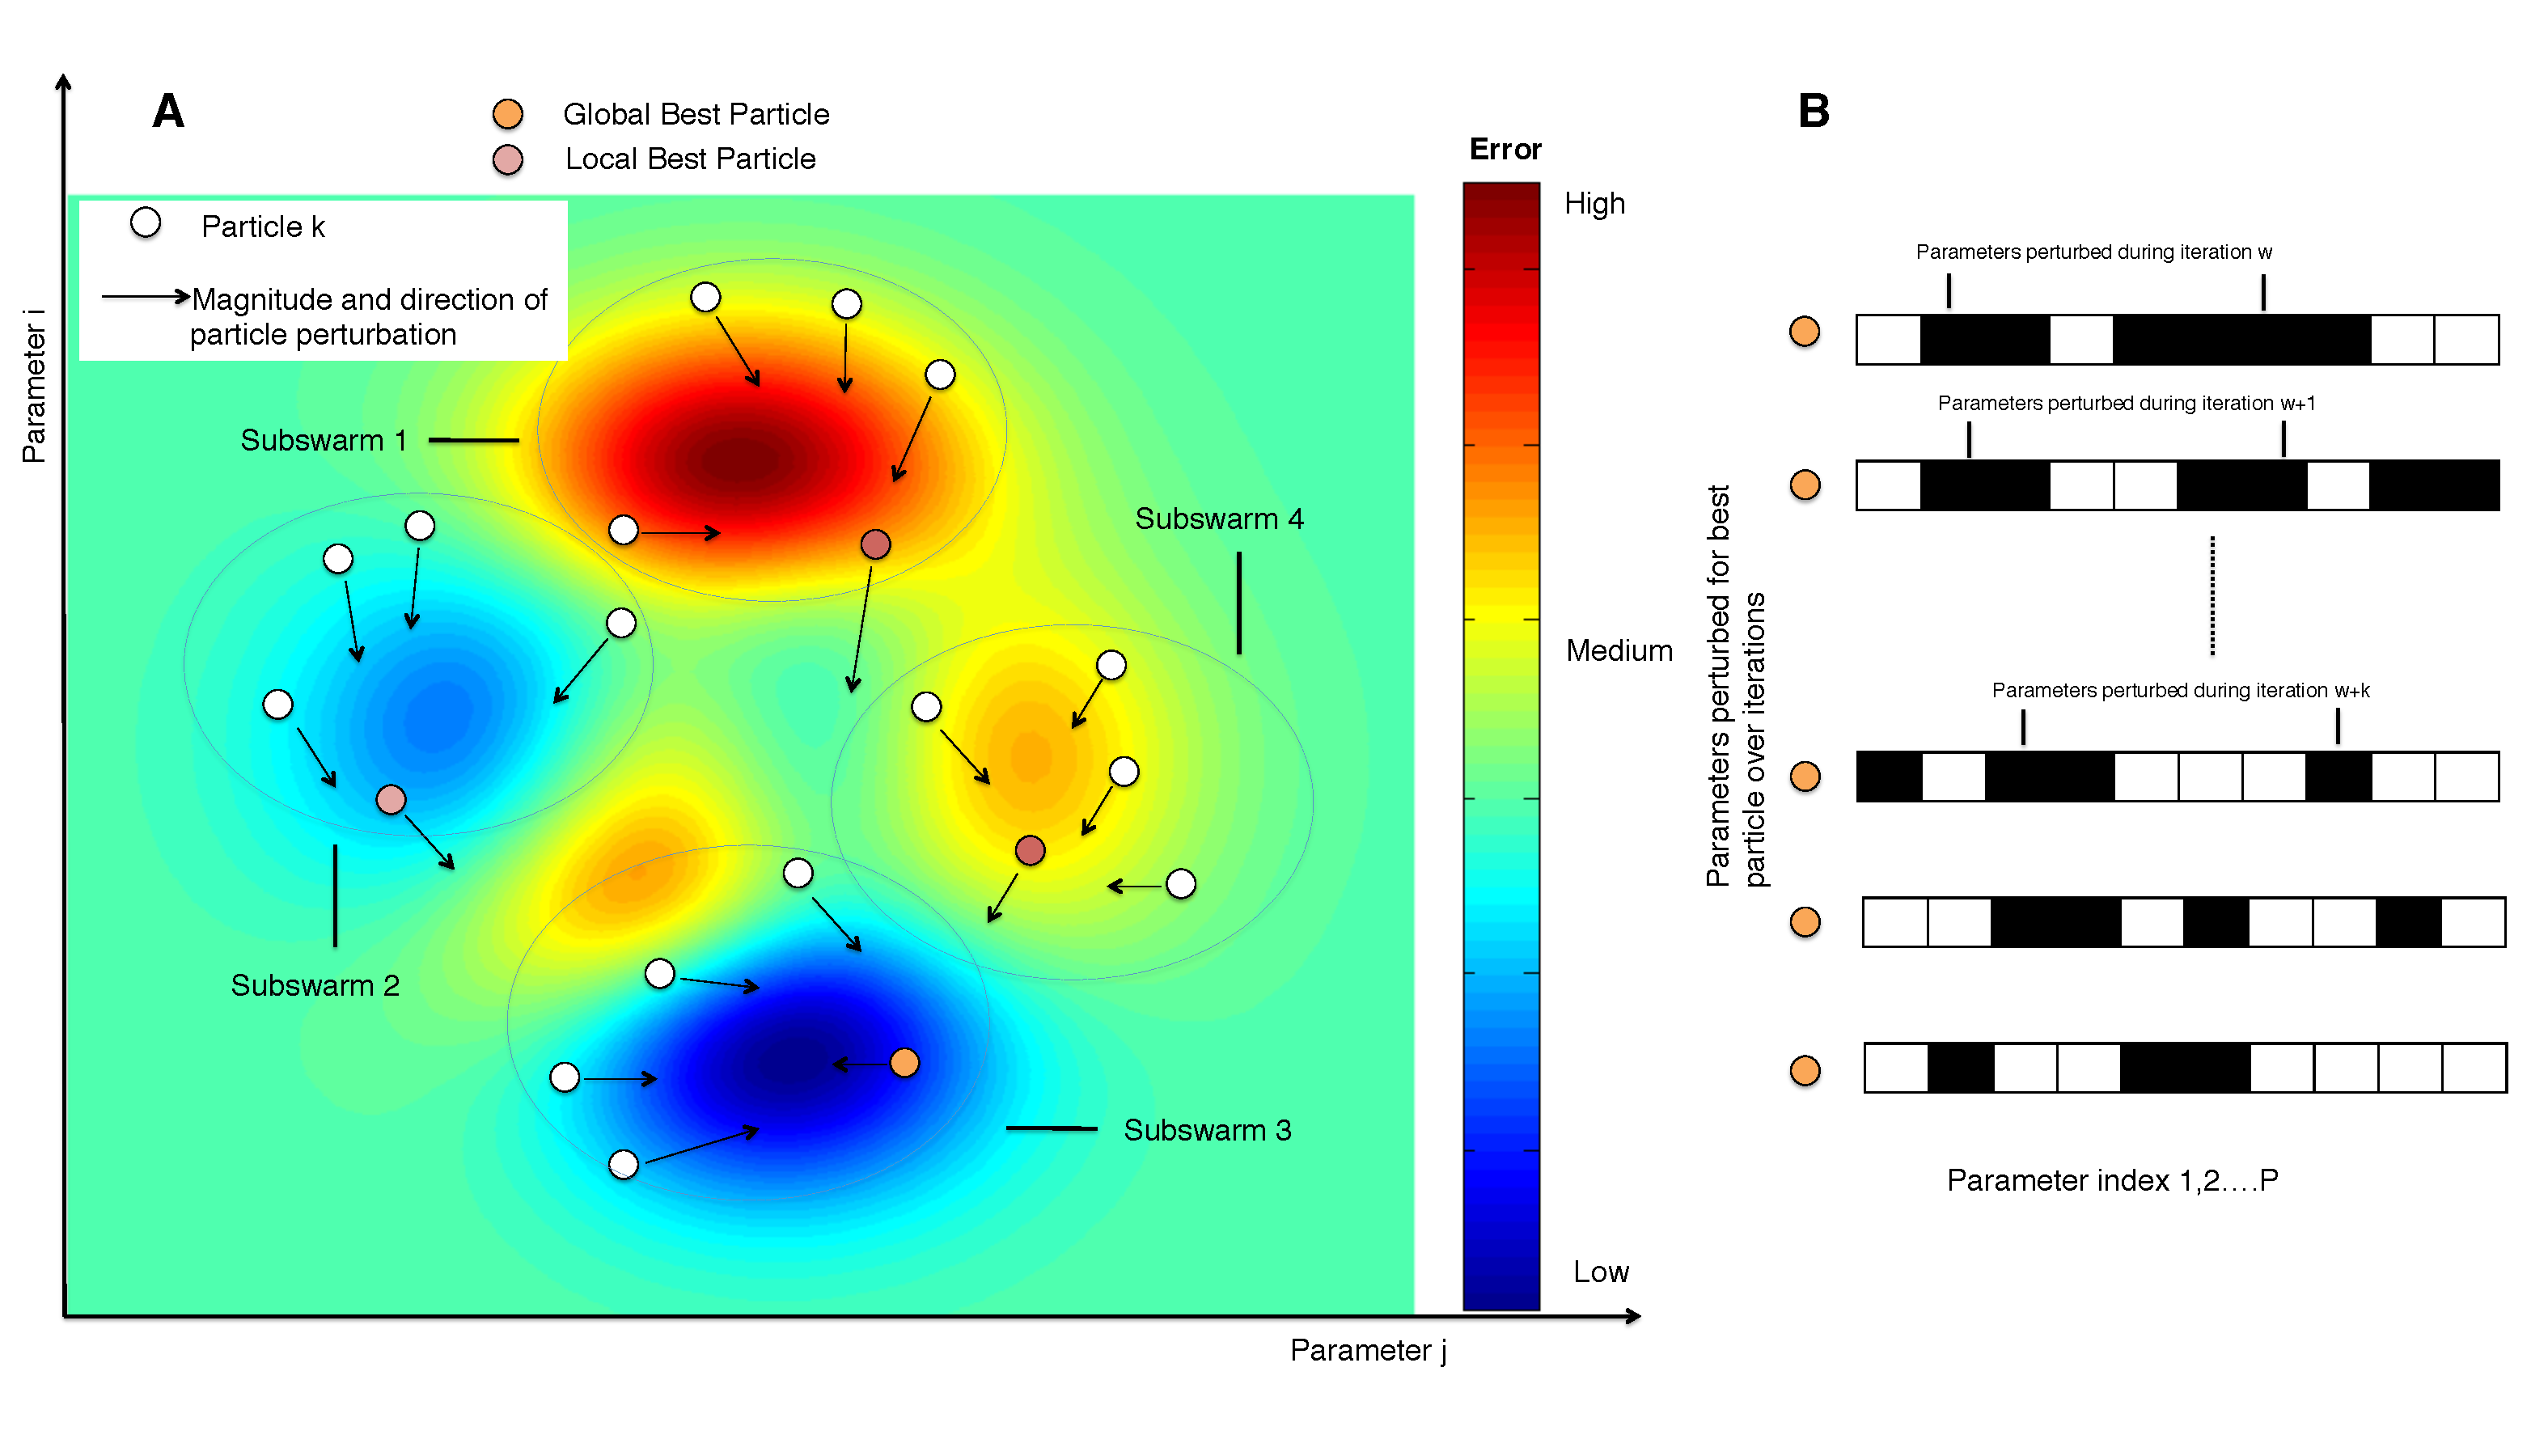
\includegraphics[width=1.0\textwidth,height=0.5\textheight]{./figs/Figure_1_Algorithm.pdf}
\caption{Dynamic Optimization with Particle Swarms.\textbf{A}: Each particle represents an N dimensional parameter vector. Particles are given randomly generated initial solutions and grouped into different sub-swarms. Within each swarm the magnitude and direction of the movement a particle is influenced by the position of the best particle and also by its own experience. After every $\mathbf{g}$ number of function evaluations the particles are mixed and randomly assigned to different swarms. When the error due to the global best particle (best particle amongst all the sub-swarms - orange color) does not drop over a certain number of function evaluations, the swarm search is stopped and the search switches to a Dynamically Dimensioned Search with global best particle as the initial solution vector or candidate vector.
\textbf{B}: The candidate vector performs a greedy global search for the remaining number of function evaluations. The search neighborhood is dynamically adjusted by varying the number of dimensions that are perturbed (in black) in each evaluation step. The probability that a dimension is perturbed decreases as the number of function evaluations increase. Thus as the evaluations increase the optimality of the solution is preserved.
}\label{fig-algorithm}
\end{figure}

\clearpage

\begin{figure}[h]
\centering
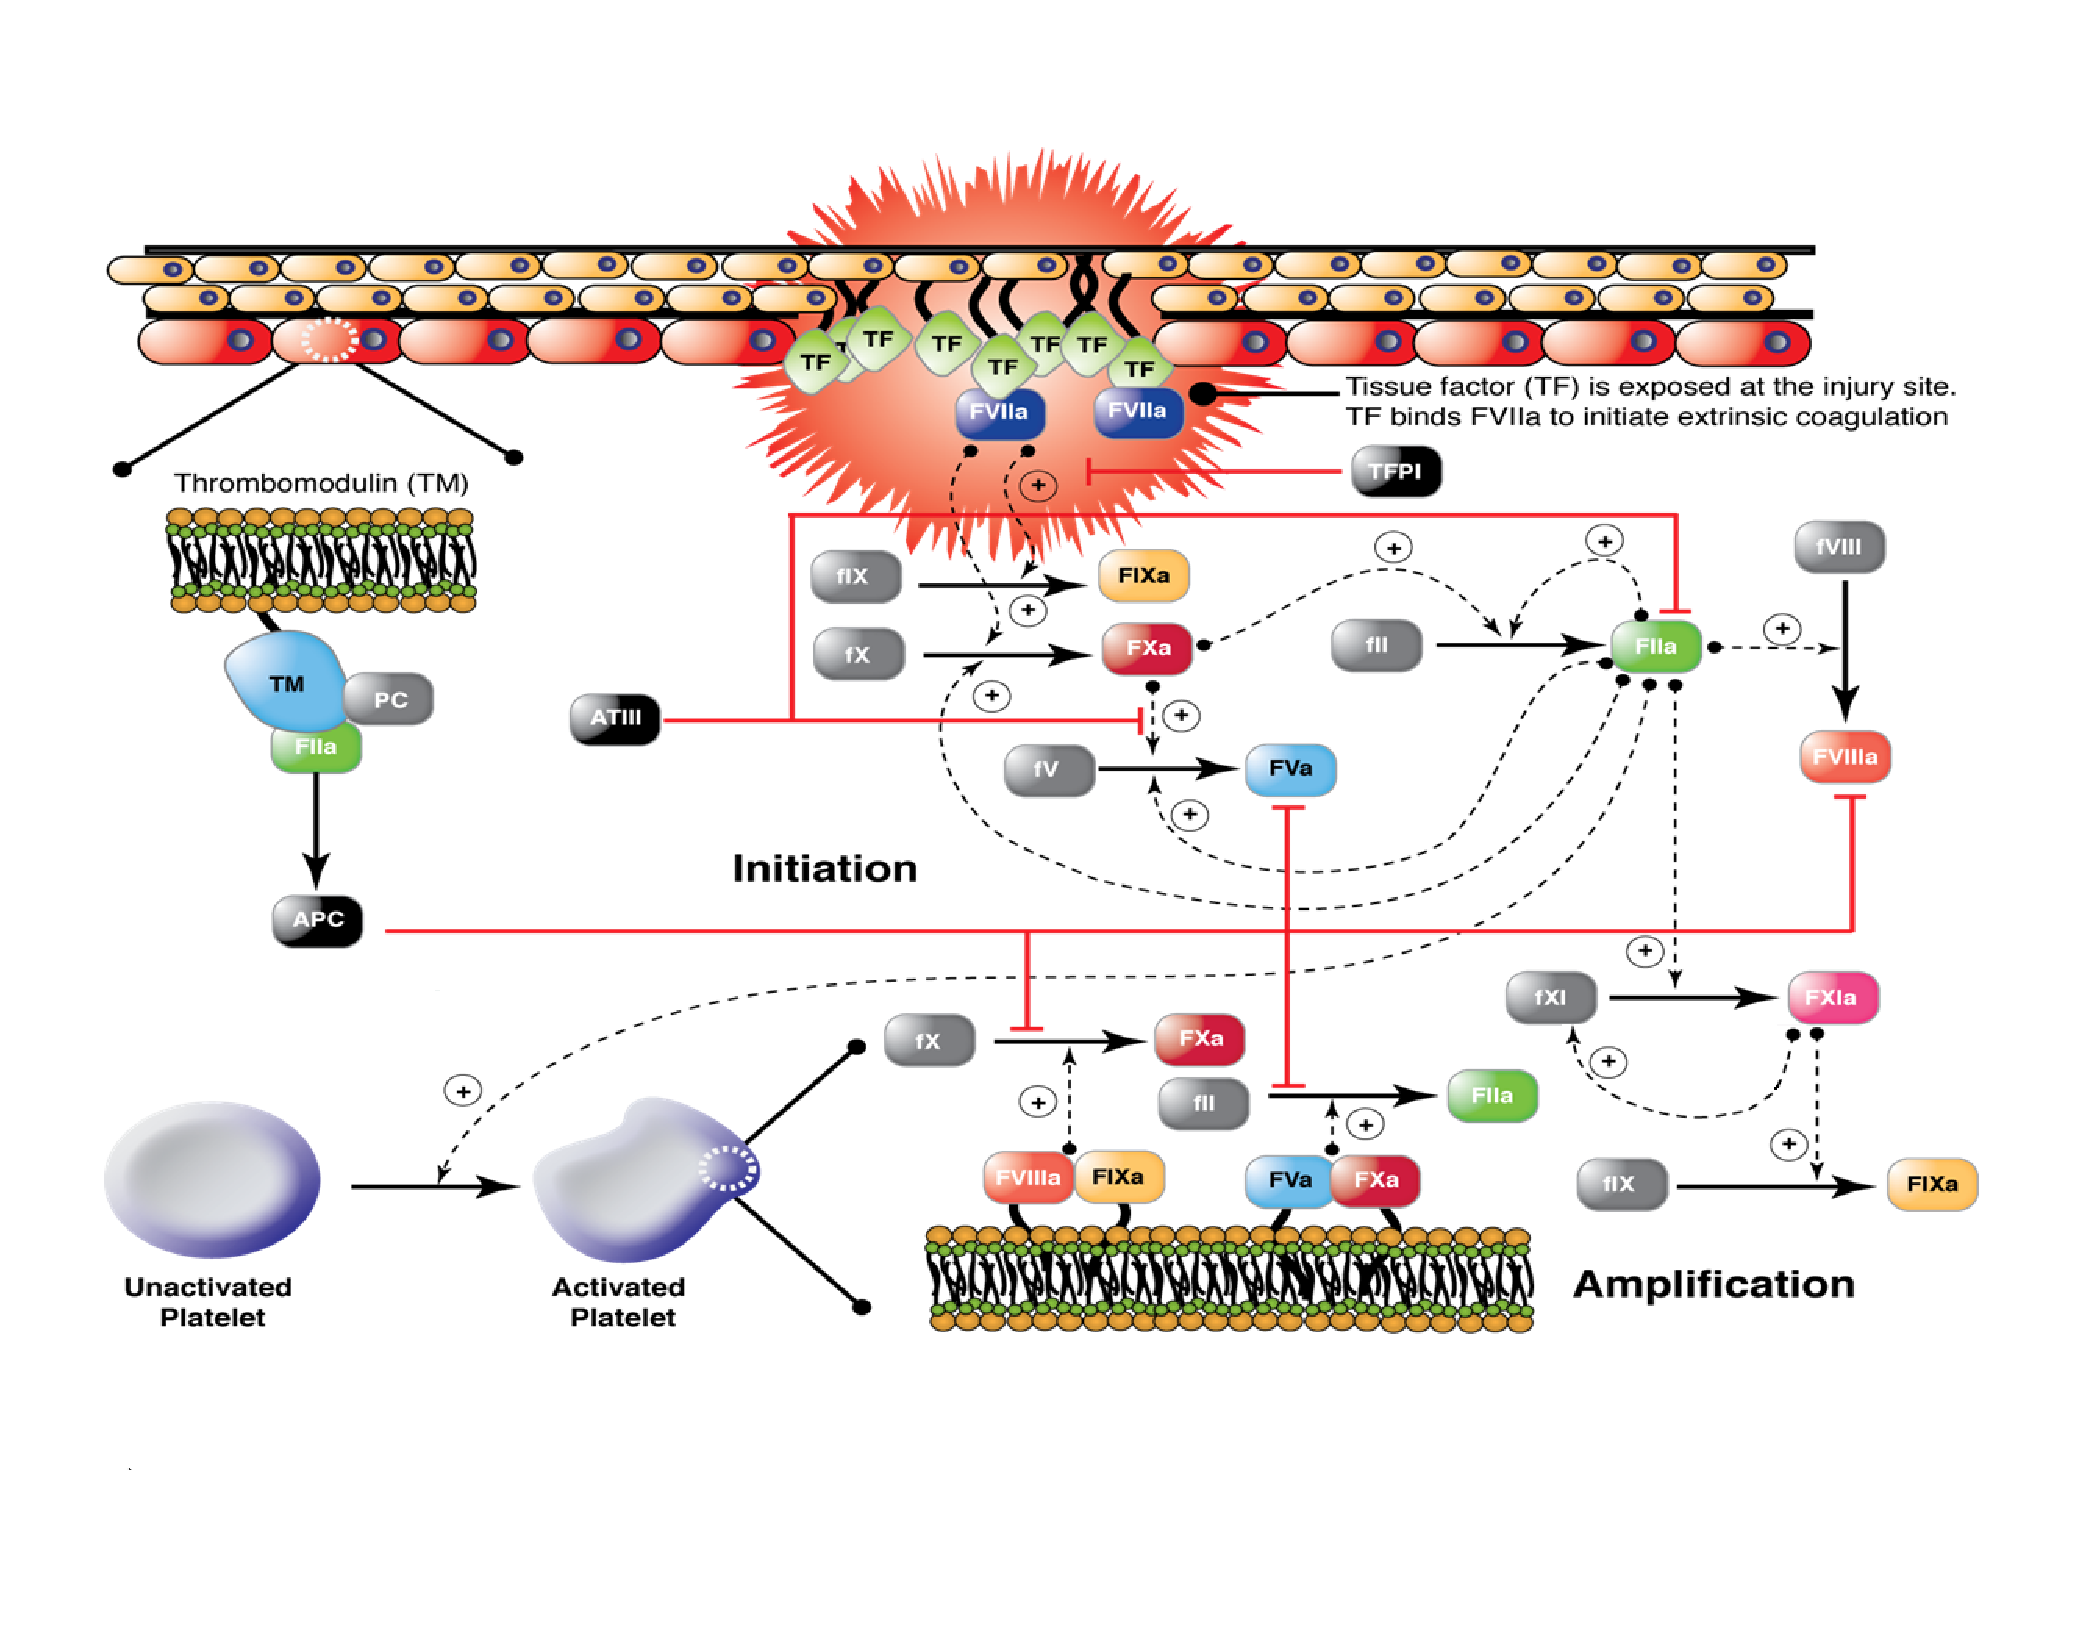
\includegraphics[width=1.00\textwidth,height=0.7\textheight]{./figs/Figure_2_CoagulationNetwork.pdf}
\caption{Schematic of the extrinsic and intrinsic coagulation cascade\cite{luan2007computationally}. Inactive zymogens upstream (grey) are activated by exposure to tissue factor (TF)  following vessel injury. Tissue factor and activated factor VIIa (FVIIa) form a complex that activates factor X (fX) and IX (fIX). FXa activates downstream factors including factor VIII (fVIII) and fIX. Factor V (fV) is primarily activated by thrombin (FIIa). In addition, we included a secondary fV activation route involving FXa. FXa and FVa form a complex (prothrombinase) on activated platelets that converts prothrombin (fII) to FIIa. FIXa and FVIIIa can also form a complex (tenase) on activated platelets which catalyzes FXa formation.  Thrombin also activates upstream coagulation factors, forming a strong positive feedback ensuring rapid activation. Tissue factor pathway inhibitor (TFPI) downregulates FXa formation and activity by sequestering free FXa and TF-FVIIa in a FXa-dependent manner. Antithrombin III (ATIII)  inhibits all proteases. Thrombin inhibits itself binding the surface protein thrombomodulin (TM). The IIa-TM complex catalyzes the conversion of protein C (PC) to activated protein C (APC), which attenuates the coagulation response by the proteolytic cleavage of fV/FVa and fVIII/FVIIIa. }\label{fig-coagulation-network}
\end{figure}

\clearpage

\begin{figure}[h]
\centering
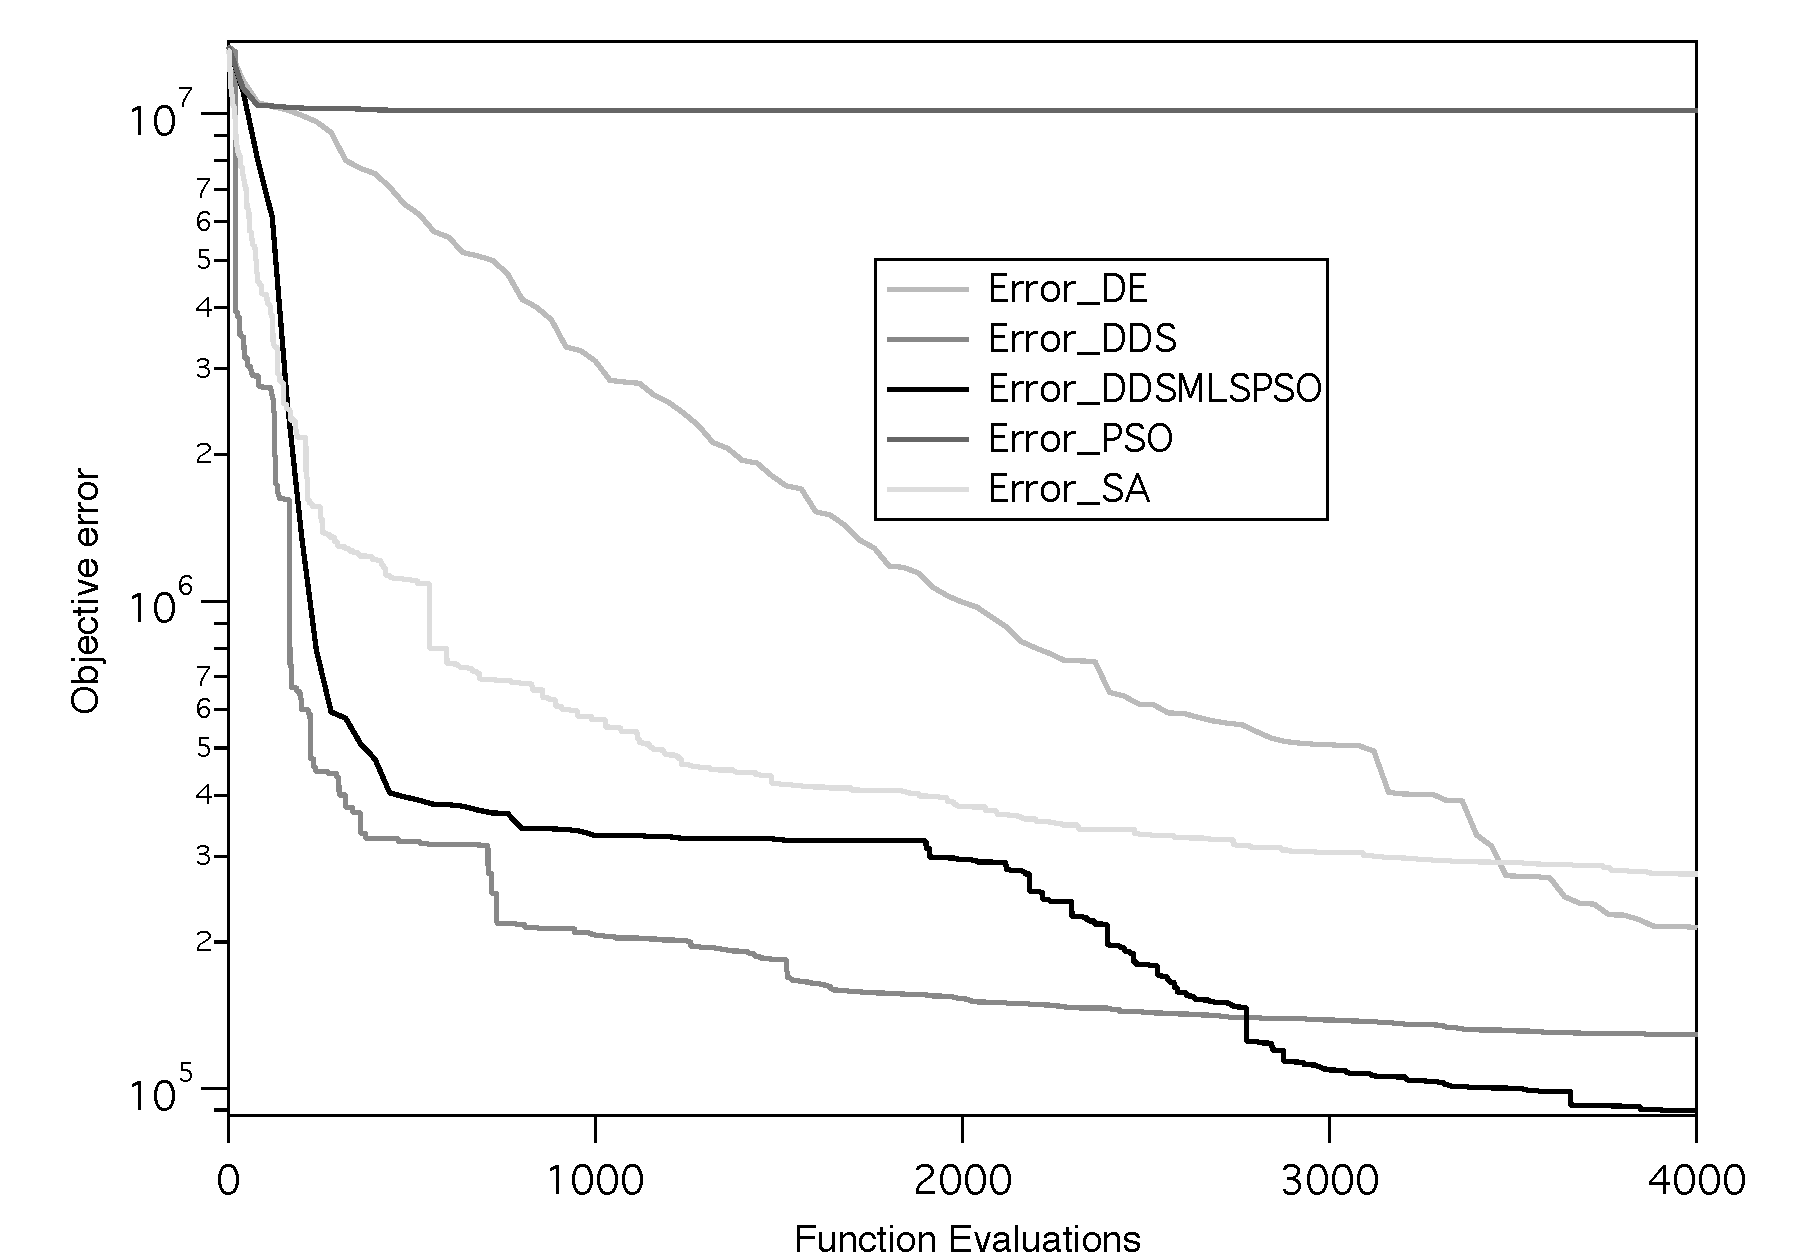
\includegraphics[width=1.0\textwidth,height=0.5\textheight]{./figs/Figure_3_Errors_convergence.pdf}
\caption{Error convergence rates of the 5 different algorithms on the coagulation model. The objective error is the mean over $N$= 25 trials. DOPS, DDS and SA have the steepest drop in error during first 300 function evaluations. Thereafter the error drop in DDS and SA remains nearly constant whereas DOPS continues to drops further. At the end of 4000 function evaluations DOPS attains the lowest error. The next best estimate using DDS is nearly 3 times greater than the lowest error using DDS.
}\label{fig-convergence}
\end{figure}

\clearpage

\begin{figure}[h]
\centering
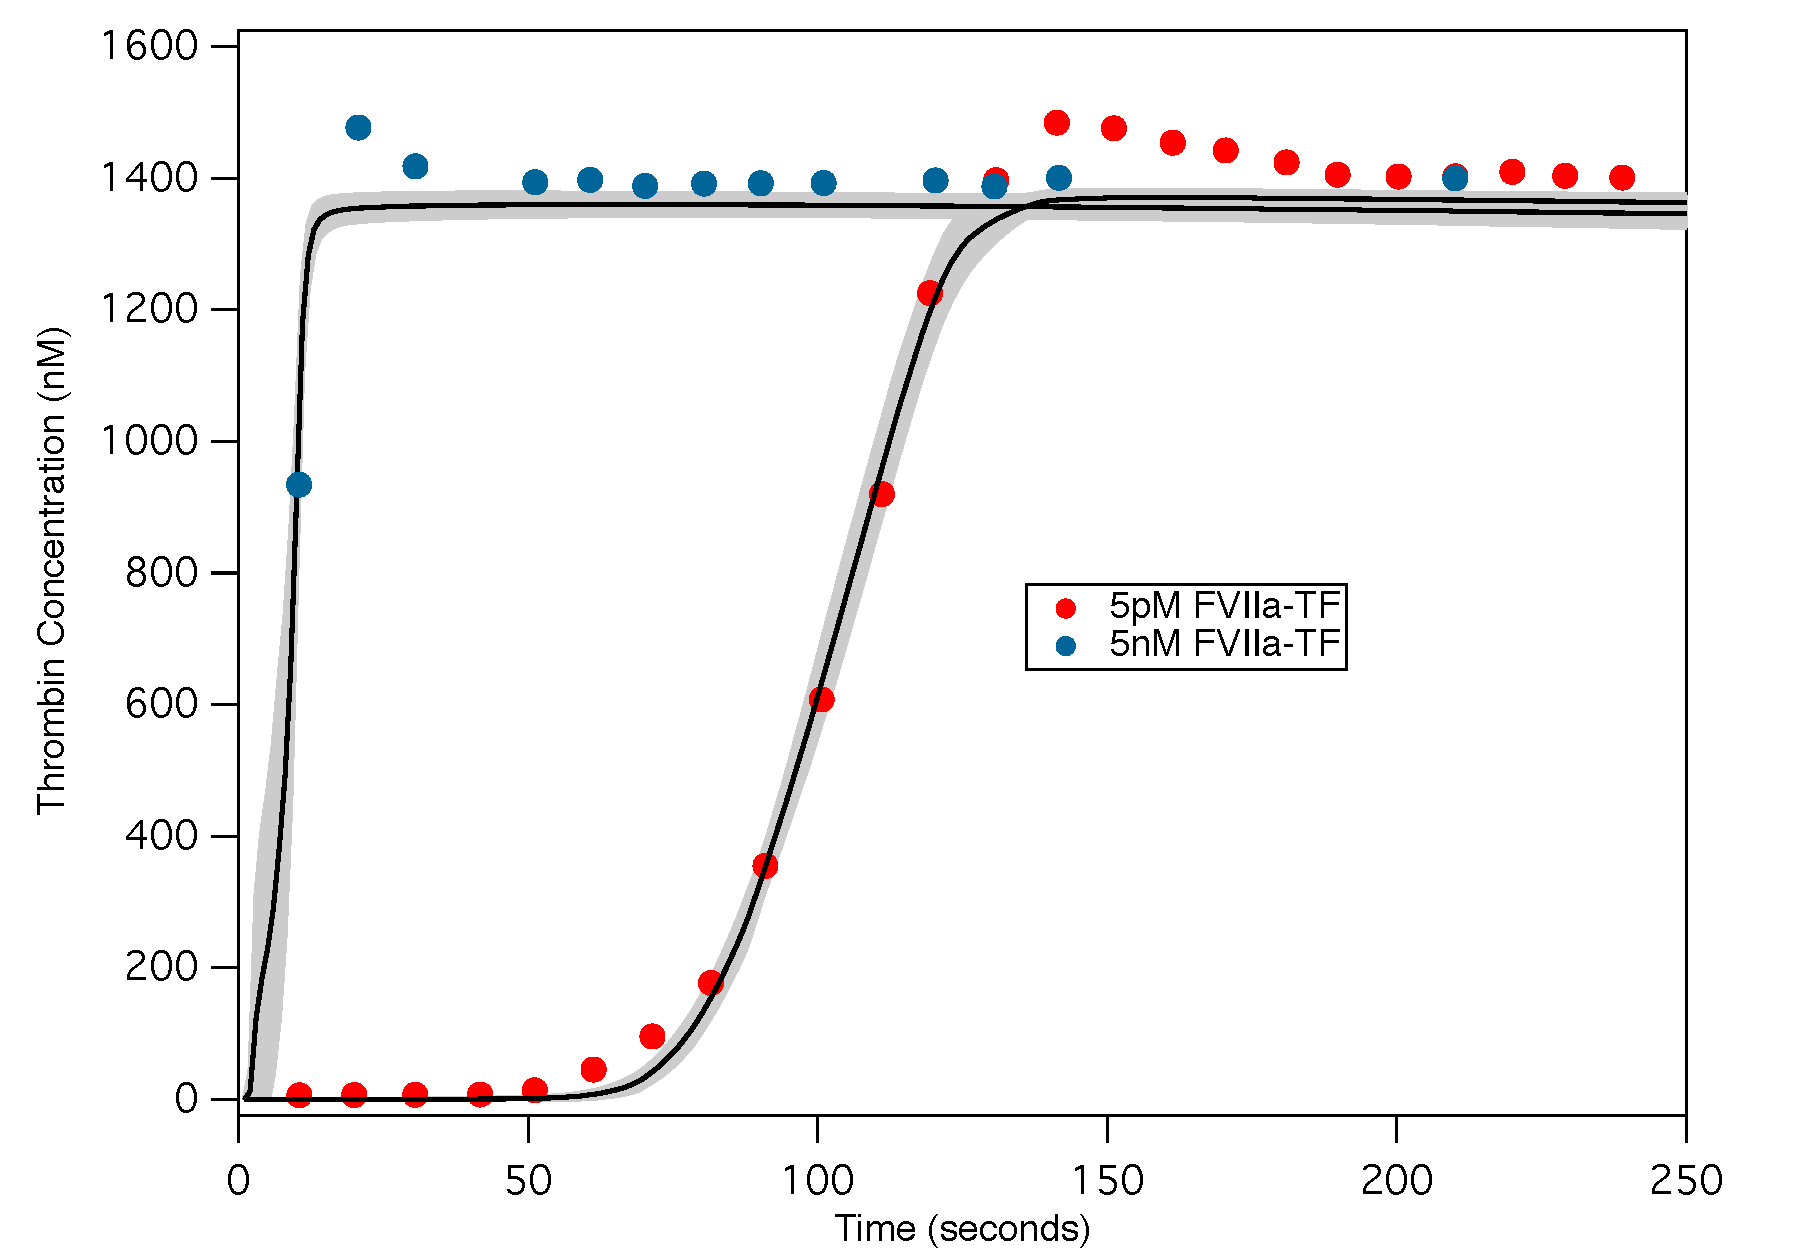
\includegraphics[width=1.0\textwidth,height=0.5\textheight]{./figs/Figure_4_Sim_Train_E1_E5.pdf}
\caption{Model fits on experimental data using DDSMLSPSO. The model parameters were estimated using DOPS. Solid black lines indicate the simulated mean thrombin concentration using parameter vectors from $N$= 25 trials. The grey shaded region represents the 99\% confidence estimate of the mean simulated thrombin concentration. The experimental data is reproduced from the synthetic plasma assays of Mann and co-workers. Thrombin generation is initiated by adding Factor VIIa-TF (5nM - Red and 5pM - Green) to synthetic plasma containing 200 $\mu$mol/L of phospholipid vesicles (PCPS) and a mixture of coagulation factors (II,V,VII,VIII,IX,X and XI) at their mean plasma concentrations.
}\label{fig-train}
\end{figure}

\clearpage

\begin{figure}[h]
\centering
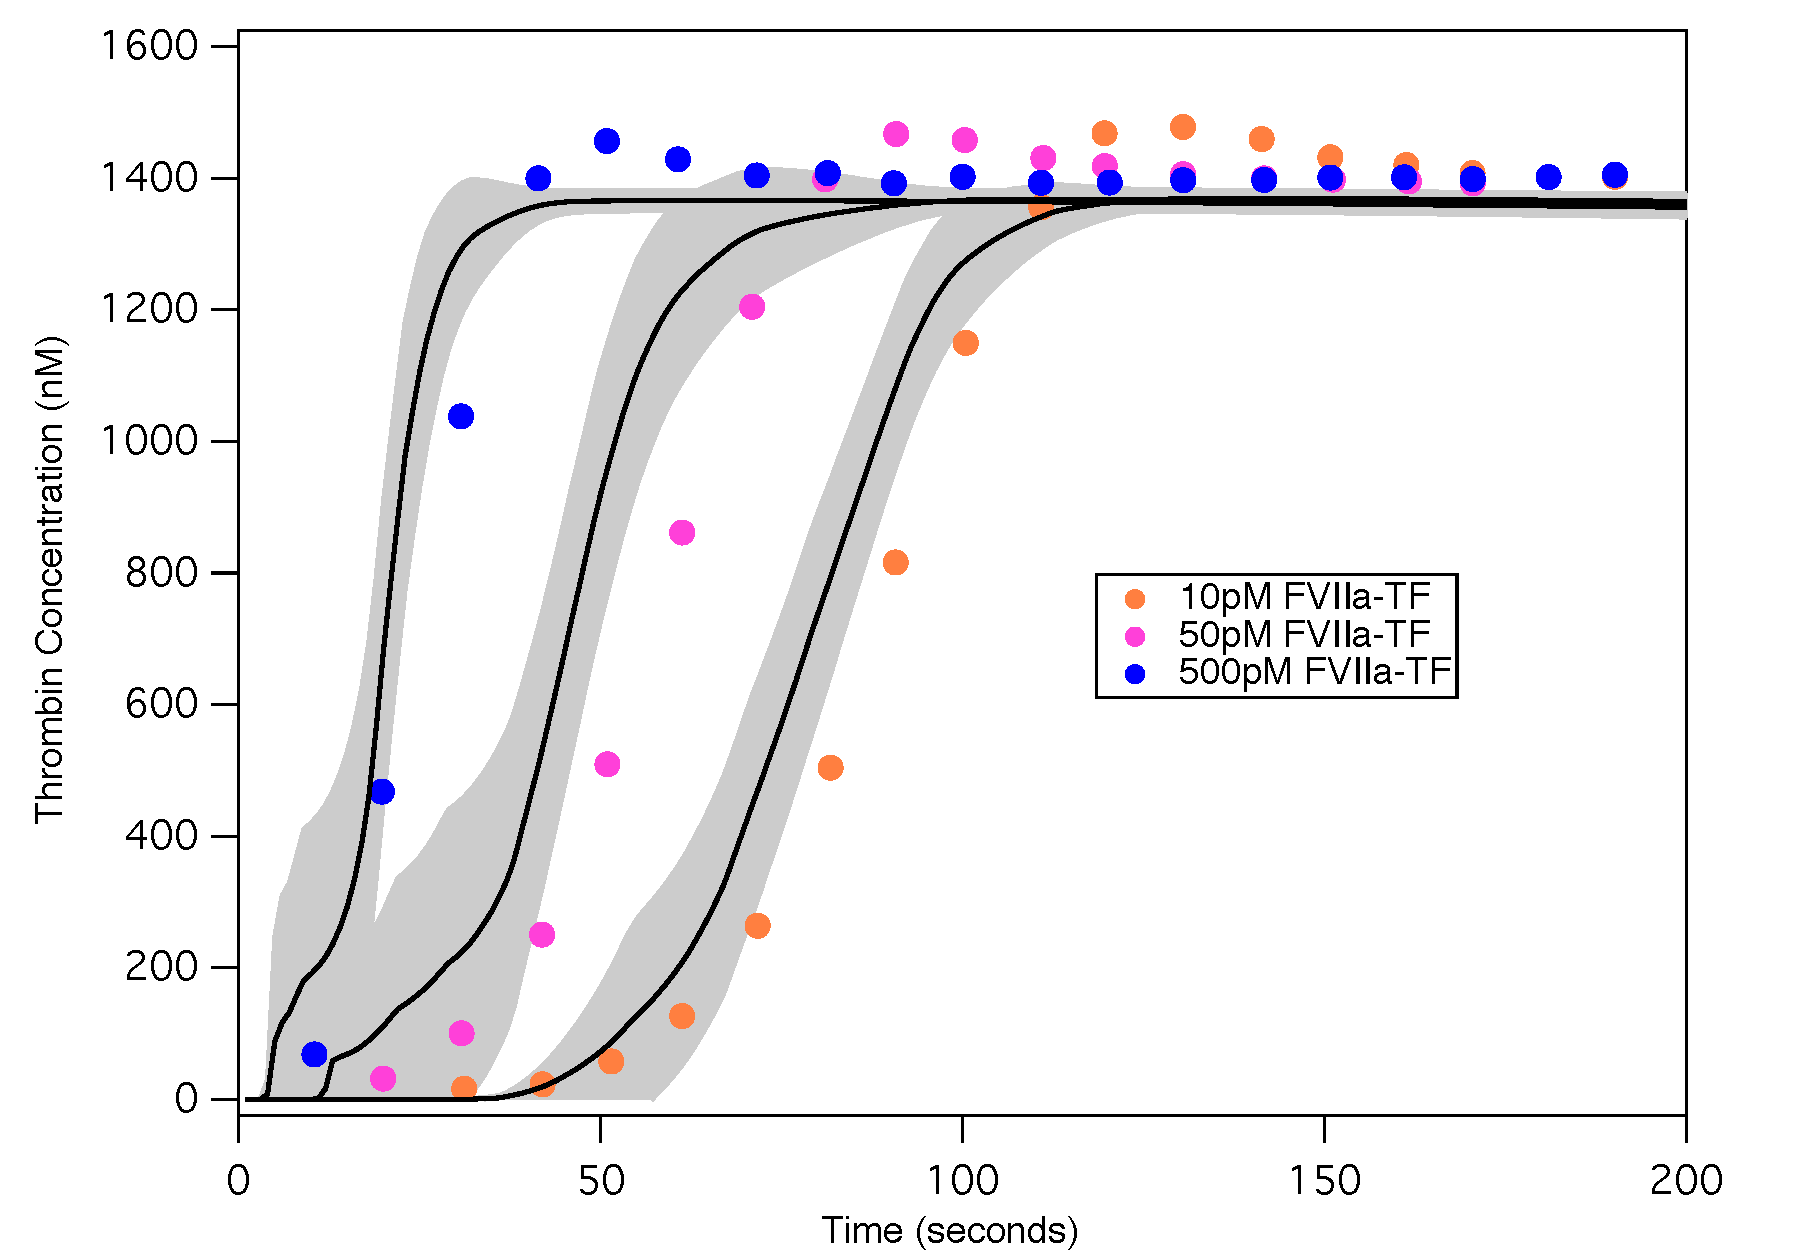
\includegraphics[width=1.0\textwidth,height=0.5\textheight]{./figs/Figure_5_Sim_Validate_E2_E4_E6.pdf}
\caption{Model predictions on unseen experimental data using parameters obtained from DOPS. The parameter estimates that were obtained using DOPS were tested against data that was not used in the model training. Solid black lines indicate the simulated mean thrombin concentration using parameter vectors from $N$= 25 trials. The grey shaded region represents the 99\% confidence estimate of the mean simulated thrombin concentration. The experimental data is reproduced from the synthetic plasma assays of Mann and co-workers. Thrombin generation is initiated by adding Factor VIIa-TF (500pM - Blue, 50pM - Pink and 10pM - Orange respectively) to synthetic plasma containing 200 $\mu$mol/L of phospholipid vesicles (PCPS) and a mixture of coagulation factors (II,V,VII,VIII,IX,X and XI) at their mean plasma concentrations.
}\label{fig-validation}
\end{figure}

\begin{figure}[ht]
\centering
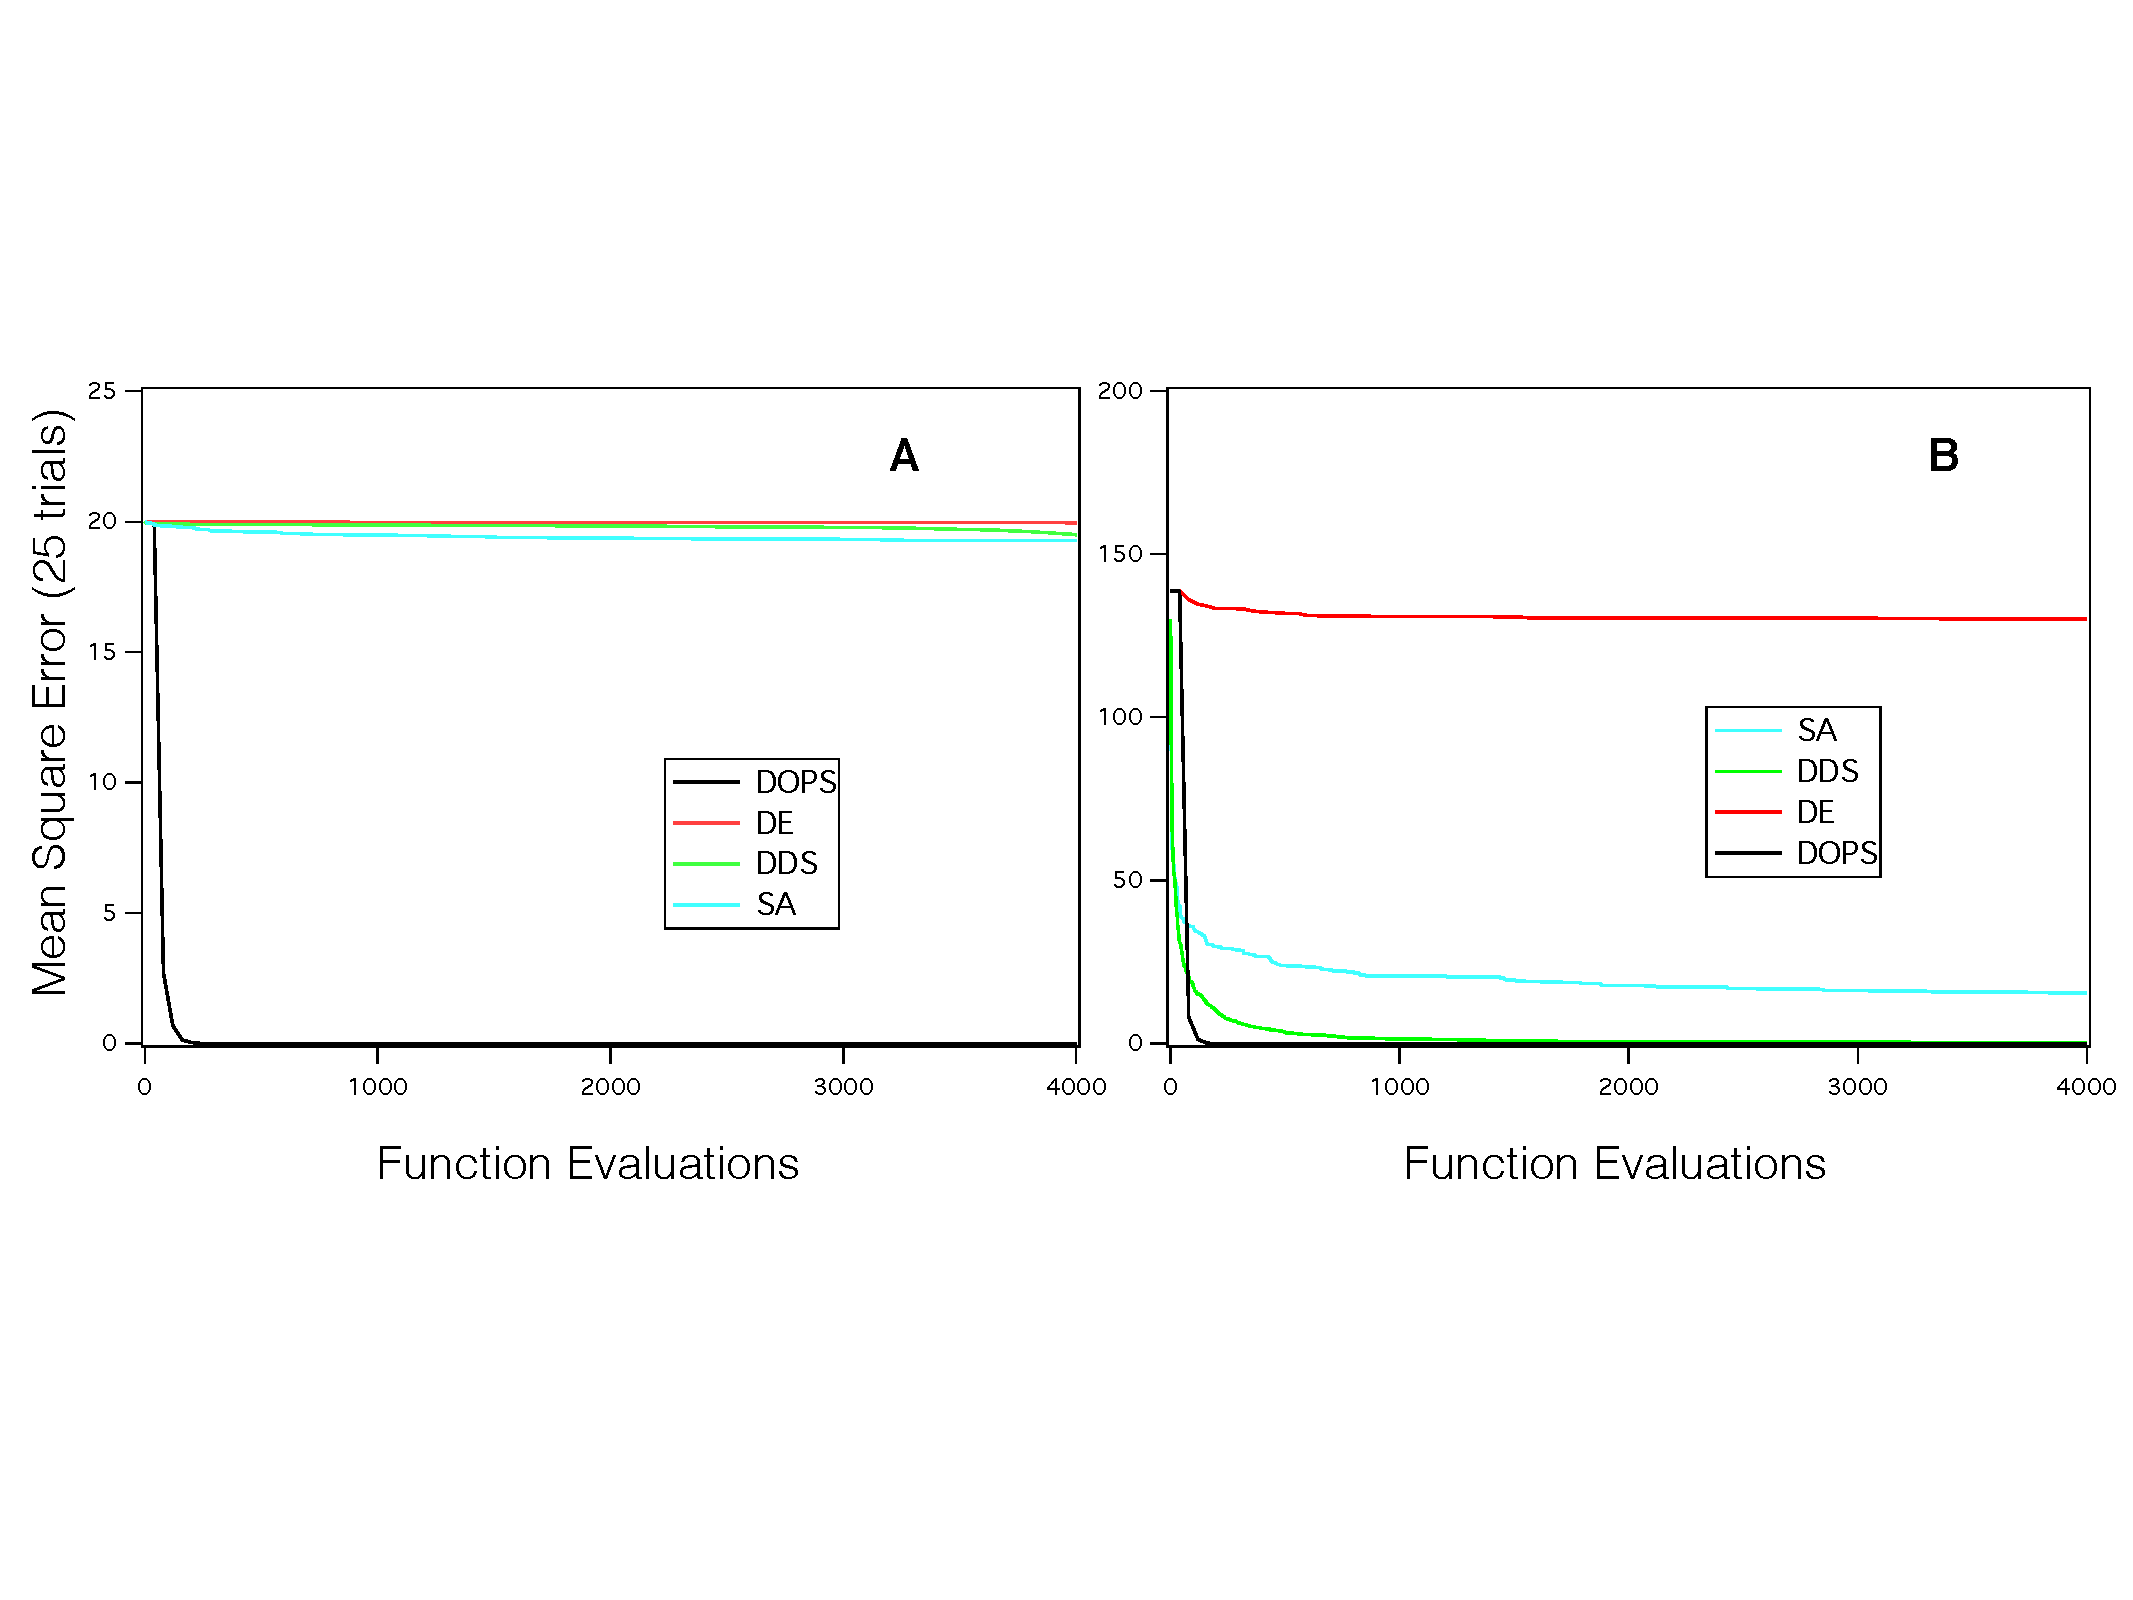
\includegraphics[width=1.00\textwidth,height=0.5\textheight]{./figs/Figure_6_Ackley_Rast}
\caption{Error convergence on 300 dimensional Ackley function and Rastrigin function. \textbf {(A)} Error convergence of 4 different meta-heuristics on 300 dimensional Ackley function \textbf {(B)} Error convergence of 4 different meta-heuristics on 300 dimensional Rastrigin function
}\label{fig-testfunctions}
\end{figure}

\begin{figure}[ht]
\centering
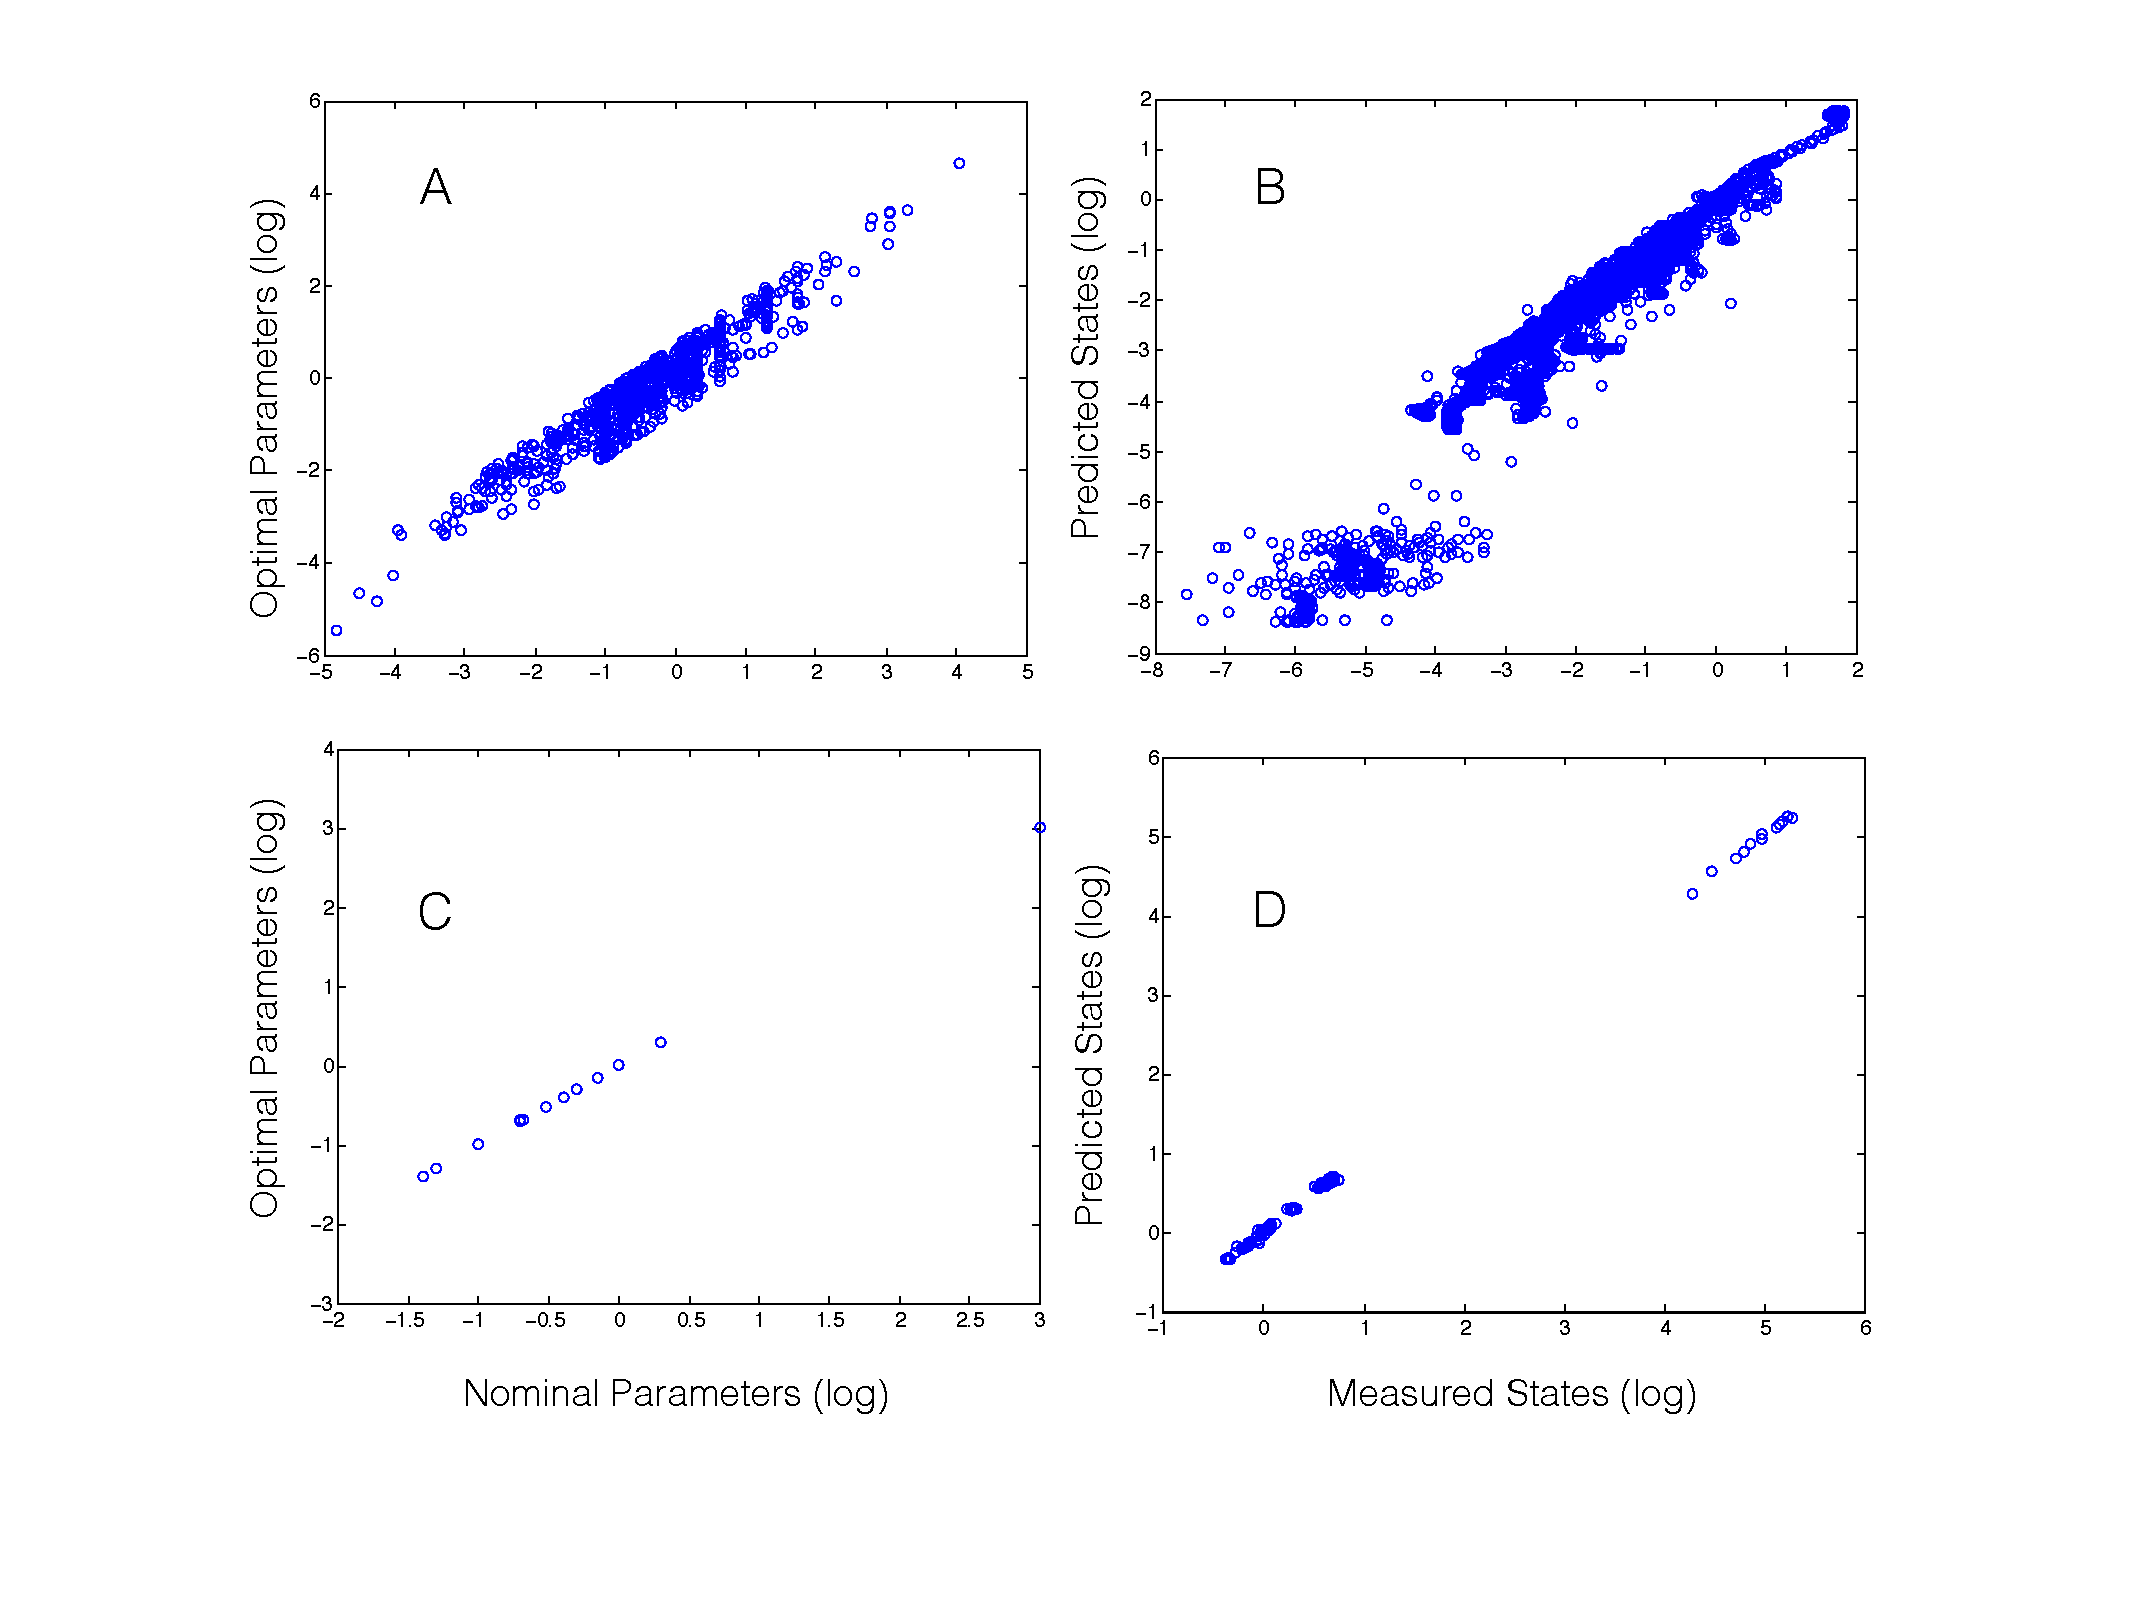
\includegraphics[width=1.00\textwidth,height=0.7\textheight]{./figs/Figure_B1_B4_params_measuredstates}
\caption{ \textbf {(A)} Difference between nominal and optimal parameters for problem B1: Genome wide kinetic model of \textit{S.cerevisiae} with 1759 unknown parameters. \textbf {(B)} Difference between experimental (measured) data and data simulated with optimal parameters for problem B1: Genome wide kinetic model of \textit{S.cerevisiae} with 1759 unknown parameters. \textbf {(C)} Difference between nominal and optimal parameters for problem B4: Metabolic model of Chinese  Hamster Ovary Cells (CHO) cells with 117 parameters. \textbf {(D)} Difference between experimental (measured) data and data simulated with optimal parameters for problem B4: Metabolic model of Chinese  Hamster Ovary Cells (CHO) cells with 117 parameters.
}\label{fig-benchmark}
\end{figure}

\begin{figure}[ht]
\centering
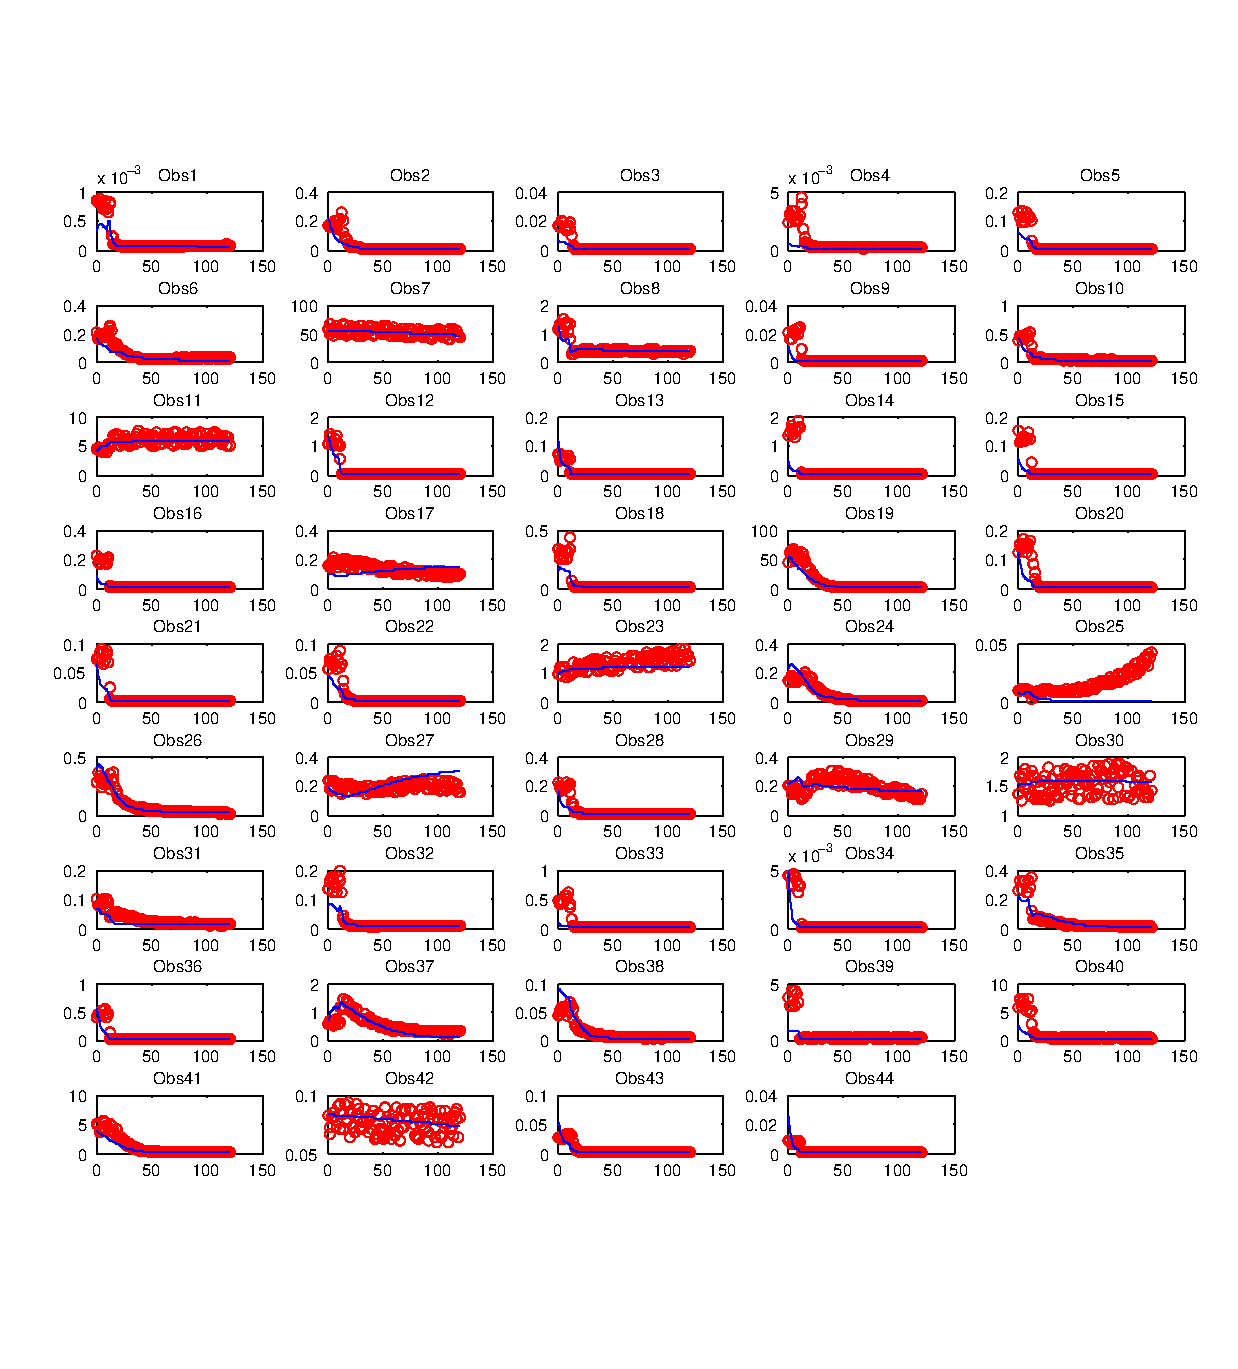
\includegraphics[width=1.00\textwidth,height=0.7\textheight]{./figs/B1_sims.pdf}
\caption{\textbf {(Data fits for Problem B1)} Pseudo-experimental data (red circles) vs. optimal solution obtained using DOPS (solid blue lines) for the 44 observed states. X axis: time [s]; Y axis: metabolite concentrations [mM].
}\label{fig-sims-b1}
\end{figure}

\begin{figure}[ht]
\centering
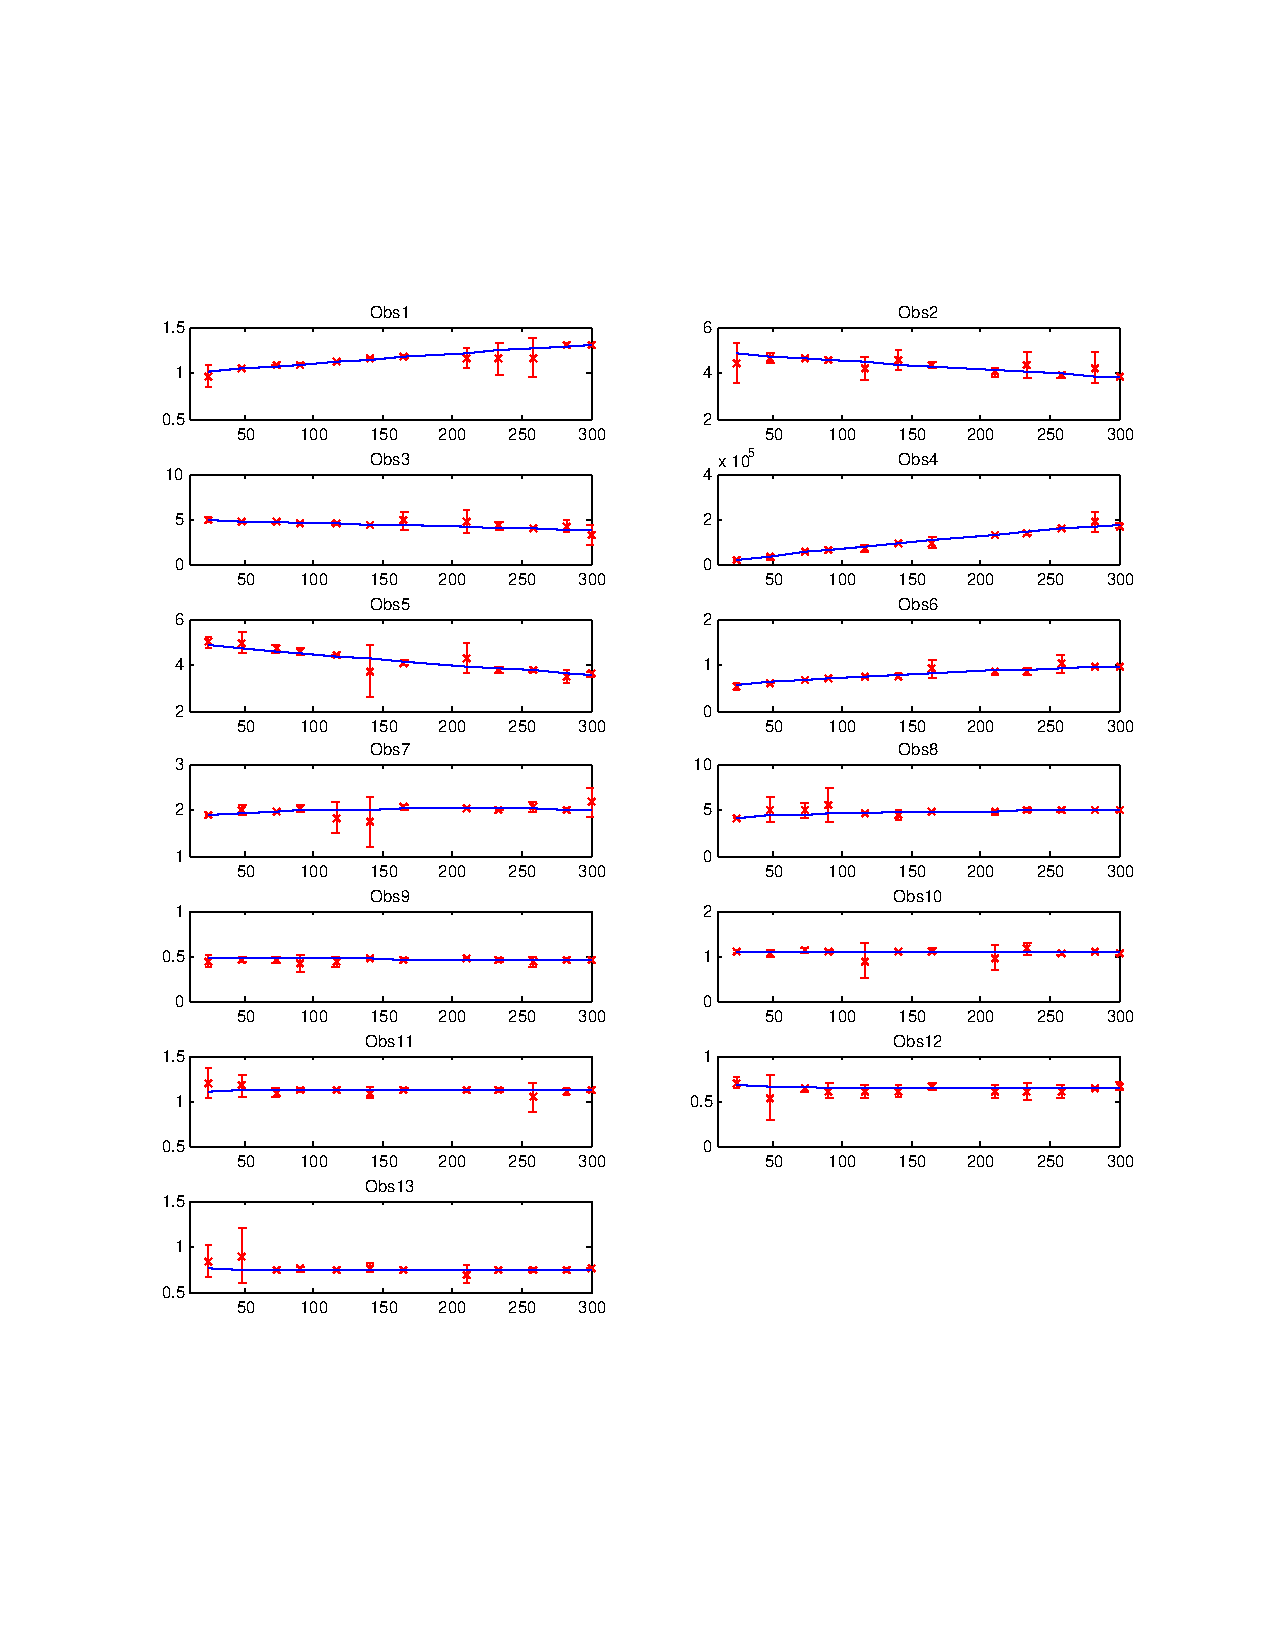
\includegraphics[width=1.00\textwidth,height=0.7\textheight]{./figs/FigB4_sims.pdf}
\caption{\textbf {(Data fits for Problem B4)} Pseudo-experimental data (red x) vs. optimal solution obtained using DOPS (solid blue lines) for the 13 observed states. X axis: time [s]; Y axis: metabolite concentrations [mM].
}\label{fig-sims-b4}
\end{figure}


%\bibitem[Saltelli \em{et~al.}(2010)Saltelli, Annoni, Azzini, Campolongo, Ratto,
  %and Tarantola]{Saltelli:2010}
%Saltelli, A.; Annoni, P.; Azzini, I.; Campolongo, F.; Ratto, M.; Tarantola, S.
%\newblock Variance based sensitivity analysis of model output. Design and
  %estimator for the total sensitivity index.
%\newblock {\em Comput. Phys. Commun.} {\bf 2010}, {\em 181},~259--270.

%\end{thebibliography}

\clearpage

% Supplemental figures -
% Set the S-
\renewcommand\thefigure{S\arabic{figure}}
\renewcommand\thetable{T\arabic{table}}
\renewcommand\thepage{S-\arabic{page}}
\renewcommand\theequation{S\arabic{equation}}

% Reset the counters -
\setcounter{equation}{0}
\setcounter{table}{0}
\setcounter{figure}{0}
\setcounter{page}{1}




\end{document}
